% !TeX program = xelatex
\documentclass[UTF8,a4paper,12pt]{ctexart}

% ===================== 核心包 =====================
\usepackage{amsmath, amssymb, amsfonts, amsthm}
\usepackage{graphicx}
\usepackage{geometry}
\usepackage{fancyhdr}
\usepackage{titlesec}
\usepackage{hyperref}
\usepackage{xcolor}
\usepackage{booktabs}
\usepackage{caption}
\usepackage{enumitem}
\usepackage{tocloft}
\usepackage{appendix}
\usepackage{listings}
\usepackage{algorithm}
\usepackage{algpseudocode}
\usepackage{float}
\usepackage{multirow}
\usepackage{subcaption}
\usepackage{tabularx}
\usepackage{setspace}
\usepackage{indentfirst}

% ===================== 暖色调配色 =====================
\definecolor{warmprimary}{RGB}{175,90,55}       % 暖陶土色 —— 主标题、页眉线
\definecolor{warmaccent}{RGB}{195,125,70}      % 暖琥珀色 —— 证明、注
\definecolor{warmlight}{RGB}{235,210,190} % 浅暖色 —— 背景点缀
\definecolor{warmdark}{RGB}{140,65,35}   % 深暖色 —— 强调
\definecolor{warmlink}{RGB}{160,80,50} % 暖棕链接
% 提供大写别名，避免 hyperref 在 PDF 书签中因大小写不匹配而报错
\definecolor{WARMPRIMARY}{RGB}{175,90,55}
\definecolor{WARMACCENT}{RGB}{195,125,70}

% ===================== 页面布局 =====================
\geometry{
    left=2.5cm, right=2.5cm, top=2.5cm, bottom=2.5cm,
    headsep=10pt, footskip=30pt
}
\setlength{\headheight}{18.04524pt}
\addtolength{\topmargin}{-0.0pt}
\setstretch{1.32}
\setlength{\parindent}{2em}
\setlength{\emergencystretch}{2em}

% ===================== 超链接设置 =====================
\hypersetup{
    colorlinks=true,
    linkcolor=warmlink,
    urlcolor=warmlink,
    citecolor=warmlink,
    pdfborder={0 0 0}
}

% ===================== 目录样式 =====================
\renewcommand{\contentsname}{\makebox[\linewidth][c]{\color{warmprimary}\bfseries\Large 目\quad 录}}
\renewcommand{\cfttoctitlefont}{\Large\bfseries}

% ===================== 章节标题样式 =====================
\titleformat{\section}
  {\normalfont\centering\Large\bfseries\color{warmprimary}}
  {\thesection}{1em}{}

\titleformat{\subsection}
  {\normalfont\large\bfseries\color{warmprimary}}
  {\thesubsection}{1em}{}

\titleformat{\subsubsection}
  {\normalfont\normalsize\bfseries\color{warmprimary}}
  {\thesubsubsection}{1em}{}

\titleformat{\paragraph}
  {\normalfont\normalsize\bfseries\color{warmprimary}}
  {\theparagraph}{1em}{}

% ===================== 页眉页脚 =====================
\pagestyle{fancy}
\fancyhf{}
\fancyhead[L]{\textcolor{warmprimary}{\leftmark}}
\fancyhead[R]{\textcolor{warmprimary}{\thepage}}
\renewcommand{\headrule}{\color{warmprimary}\hrule width\textwidth height 0.7pt \vskip 1mm}

% ===================== 列表样式 =====================
\setlist[itemize]{label=\textcolor{warmprimary}{\textbullet}}
\setlist[enumerate]{label=\textcolor{warmprimary}{\textbf{\arabic*.}}}

% ===================== 图表标题样式 =====================
\captionsetup[table]{
    name = {表},
    labelfont = {color=warmprimary, bf},
    font=small, skip=8pt
}
\captionsetup[figure]{
    name = {图},
    labelformat = simple,
    labelfont = {color=warmprimary, bf},
    font=small, skip=8pt
}
\DeclareCaptionLabelSeparator{t1on}{\textbf{\textcolor{warmprimary}{: }}}
\captionsetup[algorithm]{
    name = {算法},
    labelformat = simple,
    labelfont = {color=warmprimary, bf},
    labelsep = t1on
}

% ===================== 数学符号定义 =====================
\newcommand{\R}{\mathbb{R}}
\newcommand{\Ncal}{\mathcal{N}}
\newcommand{\E}{\mathbb{E}}
\newcommand{\KL}{D_{\mathrm{KL}}}
\newcommand{\code}[1]{\texttt{#1}}

\newcommand{\norm}[1]{\left\| #1 \right\|}
\newcommand{\abs}[1]{\left| #1 \right|}
\newcommand{\pare}[1]{\left( #1 \right)}

\DeclareMathOperator*{\argmin}{argmin}
\DeclareMathOperator*{\argmax}{argmax}

% ===================== 证明/注环境 =====================
\newenvironment{pf}{
    \par\noindent\textcolor{warmaccent}{\textbf{证明}}\quad\ignorespaces
}{\qed\par}

\newenvironment{rmk}{
    \par\noindent\textcolor{warmaccent}{\textbf{注}}\quad\ignorespaces
}

% ===================== 定理类环境（本文未使用，预留） =====================
% \newtheoremstyle{colored}%
% {}{}{\itshape}{}{\color{warmprimary}\bfseries}{ }{}
% \theoremstyle{colored}
% \newtheorem{thm}{定理}[section]
% \newtheorem{defi}[thm]{定义}

% ===================== 代码风格 =====================
\lstset{
    basicstyle=\ttfamily\footnotesize,
    frame=single, framerule=0.4pt, rulecolor=\color{warmprimary},
    captionpos=b, numbers=none,
    keywordstyle=\color{warmdark},
    commentstyle=\color{gray},
    stringstyle=\color{red},
    showstringspaces=false, breaklines=true,
}

% ===================== 图片路径 =====================
\graphicspath{{../outputs/figures/}{../outputs/figures/multiseed/}{../outputs/figures/latent/}}

\begin{document}

% ===================== 封面 =====================
\begin{titlepage}
\centering
\vspace*{3.0cm}

{\zihao{2}\bfseries\color{warmprimary} 二维分布生成建模：\\[0.4cm]
VAE、扩散模型与流模型\\[0.4cm]
的实验比较\par}

\vspace{1.8cm}

{\zihao{4}韦晏洲（组长） \quad PB24000379 \quad 158\par}
\vspace{0.5cm}
{\zihao{4}黎思远 \quad PB23061257 \quad 102\par}
\vspace{0.5cm}
{\zihao{4}黄鑫源 \quad PB24010418 \quad xxx\par}

\vfill

{\zihao{4}中国科学技术大学\quad 数学建模课程大作业\par}
\vspace{0.5cm}
{\zihao{4}2026 年 6 月\par}

\vspace{1.0cm}
\end{titlepage}

% ===================== 目录 =====================
\pagenumbering{Roman}
\tableofcontents
\clearpage

% ===================== 摘要 =====================
\section*{摘\quad 要}
\addcontentsline{toc}{section}{摘要}

生成建模的核心任务是学习观测数据背后的概率分布，并能够从中采样出与真实样本统计特征相近的新样本。本文围绕二维分布生成建模这一任务，在变分自编码器（VAE）和去噪扩散概率模型（DDPM）之外，进一步引入了实值非体积保持流模型（RealNVP），对 Gaussian Mixture、Ring、Two Moons 和 Spiral 四类具有不同几何特征的二维分布展开系统的三模型对比。

在方法层面，VAE 采用编码器—解码器结构实现显式潜变量建模，以证据下界为优化目标；DDPM 通过前向加噪与反向去噪的马尔可夫过程逐步逼近数据分布；RealNVP 则利用可逆仿射耦合层直接最大化精确对数似然。本文统一了数据划分、训练协议和评价标准，在五组随机种子上完成全部实验并报告均值与标准差，以保证结论的统计可靠性。

评价体系涵盖了最大均值差异（MMD）、切片 Wasserstein 距离（SWD）、Chamfer 距离、KDE/GMM 负对数似然代理指标与模式覆盖率，同时记录了训练和采样时间。实验结果表明：RealNVP 在全部四个分布上的平均 MMD 最优（0.00047），比 VAE 低约 3.2 倍，比 DDPM 低约 3.8 倍；在 Ring 和 Two Moons 上更是三指标全优。DDPM 在 Gaussian Mixture 上的局部邻域贴合（Chamfer 0.0398）保持绝对领先，但采样耗时约为 Flow 的 7 倍。VAE 在采样速度上具有毫秒级优势，但生成质量在复杂流形上明显不足。本文还通过潜空间可视化和扩散去噪快照进一步分析了三类模型的生成机理差异，并在文末讨论了各自的适用边界与局限性。

\noindent\textbf{关键词：}生成建模；变分自编码器；扩散模型；归一化流；二维分布；分布评价；数学建模

\clearpage
\pagenumbering{arabic}

% ===================== 一、问题重述 =====================
\section{问题重述}

\subsection{问题背景}

生成建模的目标是直接从观测数据中学习其背后的概率分布 $p_{\mathrm{data}}(\mathbf{x})$，并能够从中生成新的、与训练样本在统计规律上不可区分的数据点。与判别式模型不同，生成模型关心的不是"如何划分"，而是"数据从何而来"。这一能力在图像合成、异常检测、数据增强、科学仿真以及表示学习等任务中具有广泛的应用价值。

二维分布生成建模虽然在维度上远低于真实图像数据，但具备一系列独特的优势：数据可以完整地可视化在二维平面上，几何结构差异一目了然；定量评价指标可以直接在样本层面精确计算，不需要借助 Inception 网络等外部特征提取器；训练速度快，使得大量对照实验和多轮消融研究成为可能。正因为如此，二维场景是理解和比较不同生成范式的理想受控实验平台。

当前，深度生成模型领域主要存在三种主流范式：其一是以变分自编码器（VAE）为代表的显式潜变量模型，通过编码器将数据压缩到低维潜空间再由解码器重建；其二是以去噪扩散概率模型（DDPM）为代表的逐步去噪模型，将生成过程分解为多个局部噪声预测子任务；其三是以归一化流（Normalizing Flow）为代表的精确似然模型，通过一系列可逆变换直接将简单先验分布映射到复杂数据分布。这三类模型在优化目标、生成机制和计算代价上存在本质差异，但在二维场景下尚未有将它们放在一起做公平比较的系统性工作。

\subsection{数据说明}

本文采用统一的数组式数据组织方式。数据集包含四类具有不同几何特征的二维分布：

\begin{itemize}
    \item \textbf{Gaussian Mixture}：8 个等间距分布在半径约 2.6 的圆上的高斯团簇，各向同性噪声标准差约 0.16。主要考察模型是否会发生模式丢失。
    \item \textbf{Ring}：半径约 2.2 的薄环带，径向标准差约 0.13，切向噪声约 0.03。样本集中在一维闭合流形附近，考察模型对细薄结构的保持能力。
    \item \textbf{Two Moons}：两条相互靠近但彼此分离的弯曲流形，上下各半。考察模型对局部几何间隔和流形弯曲的兼顾能力。
    \item \textbf{Spiral}：两条从中心向外扩展的螺旋臂，角度范围约 $0.25\sim4\pi$。考察模型对长程连续拓扑和全局结构一致性的学习能力。
\end{itemize}

每类分布各包含 2000 个训练样本、2000 个公开测试样本以及 2000 个隐藏测试样本。本文的主体建模与评价阶段仅使用公开的训练集和测试集，隐藏测试集仅在最终未见样本验证中使用。所有样本的坐标范围大致落在 $[-4,4]\times[-4,4]$ 内。

\begin{figure}[H]
\centering
\begin{subfigure}[b]{0.48\textwidth}
    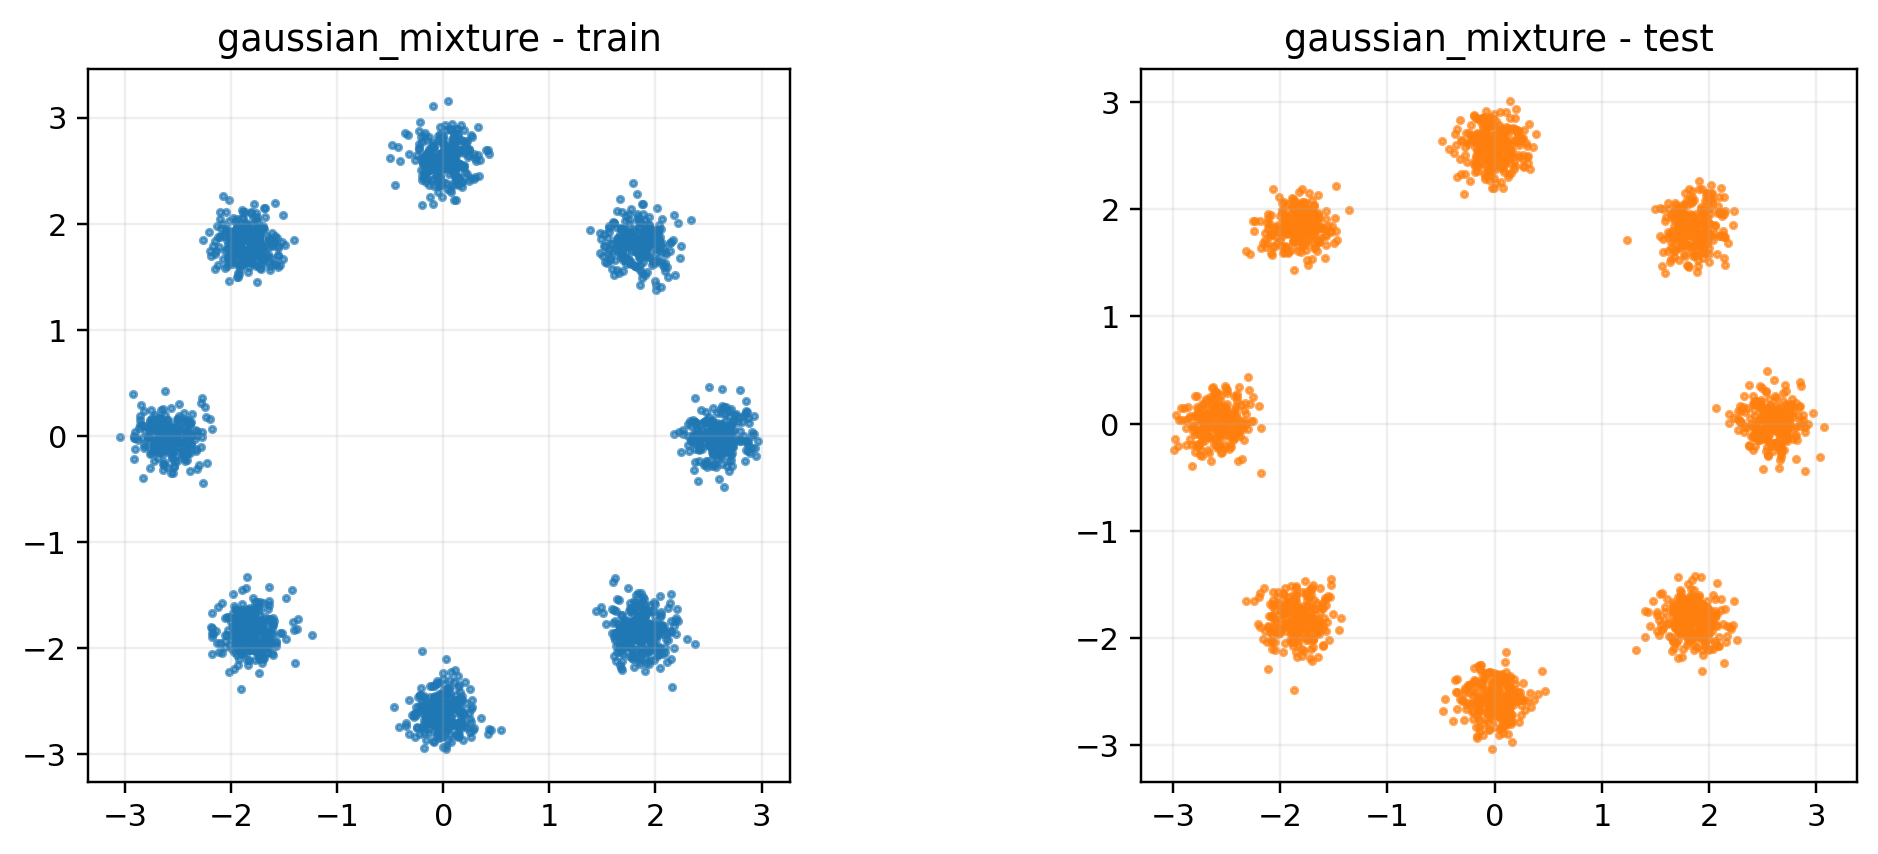
\includegraphics[width=\linewidth]{gaussian_mixture_dataset.png}
    \caption{Gaussian Mixture}
\end{subfigure}
\hfill
\begin{subfigure}[b]{0.48\textwidth}
    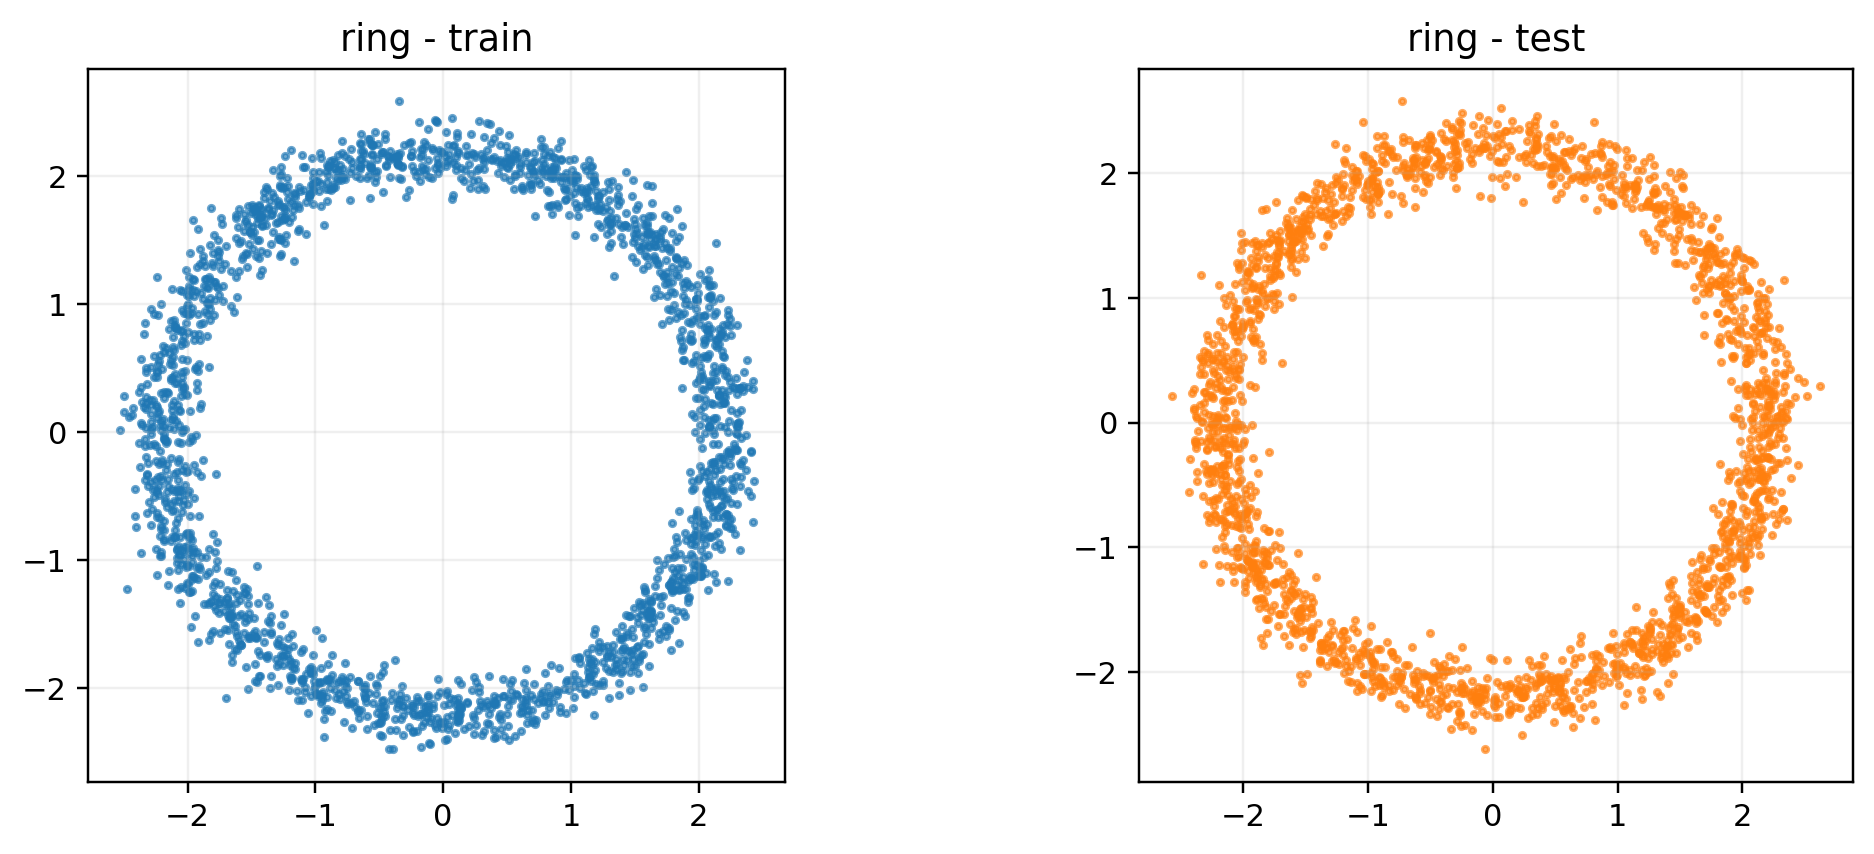
\includegraphics[width=\linewidth]{ring_dataset.png}
    \caption{Ring}
\end{subfigure}
\vspace{0.4em}
\begin{subfigure}[b]{0.48\textwidth}
    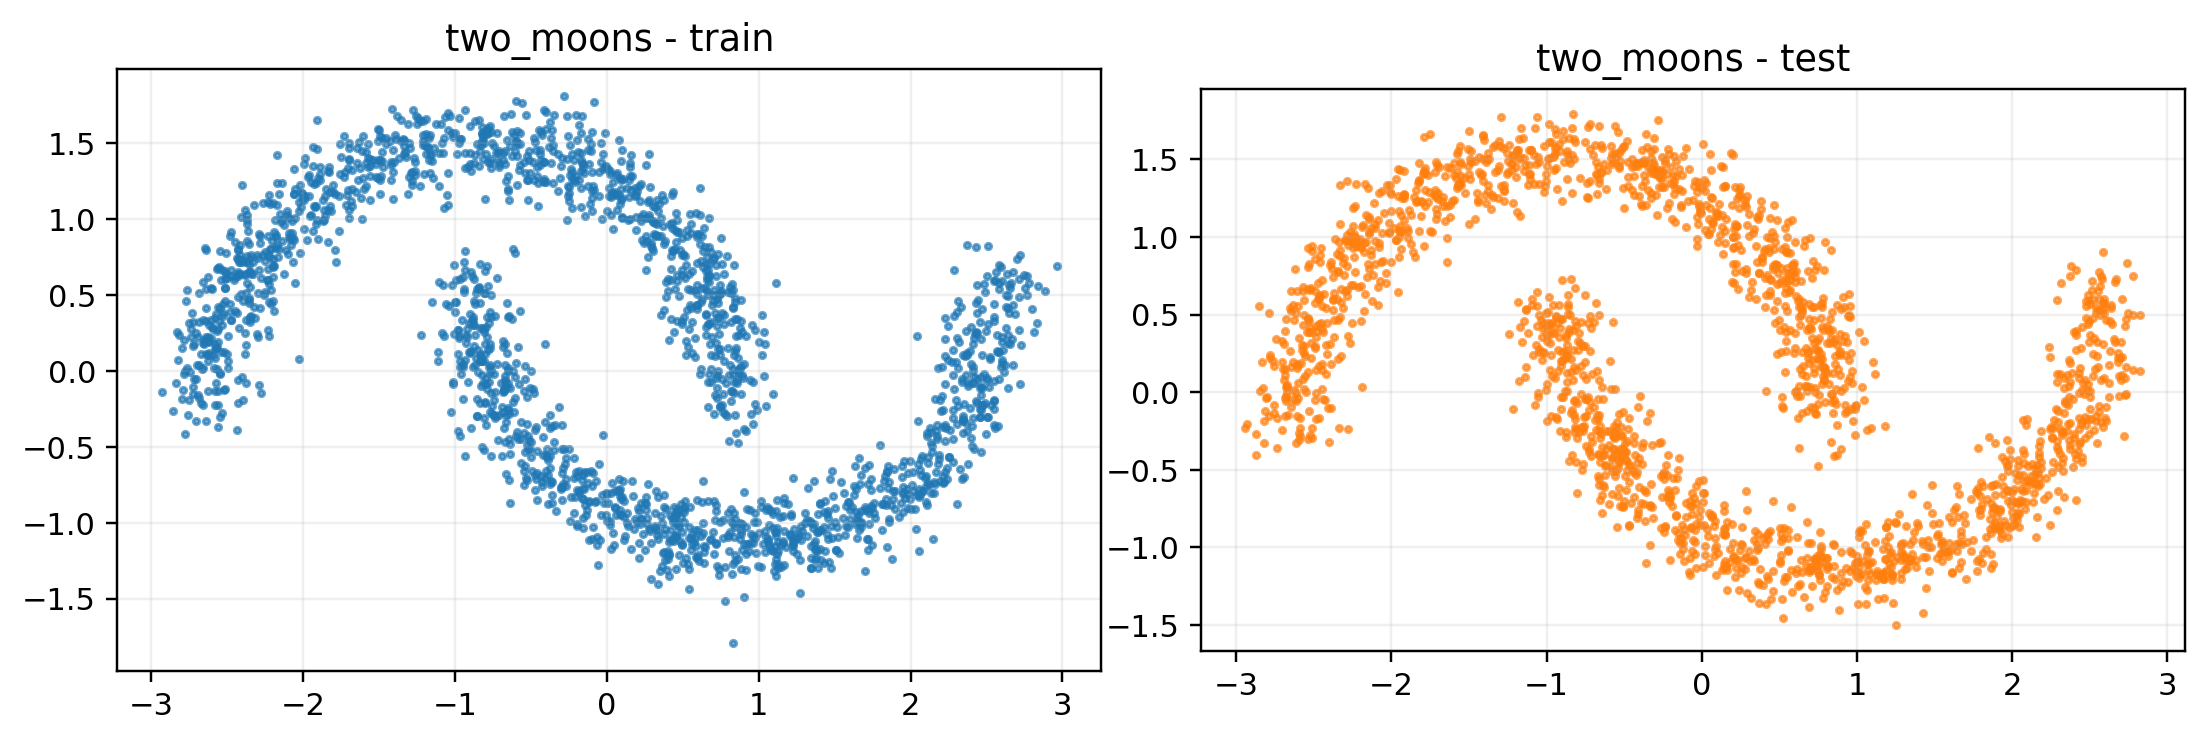
\includegraphics[width=\linewidth]{two_moons_dataset.png}
    \caption{Two Moons}
\end{subfigure}
\hfill
\begin{subfigure}[b]{0.48\textwidth}
    
\includegraphics[width=\linewidth]{spiral_dataset.png}
    \caption{Spiral}
\end{subfigure}
\caption{四类二维分布的训练集样本可视化。}
\end{figure}

从建模难度上看，四类分布形成了一个清晰的梯度：Gaussian Mixture 主要考验模式覆盖的完整性；Ring 考验低维闭合流形的保形能力；Two Moons 强调局部间隔与流形弯曲的兼顾；Spiral 则同时要求全局拓扑连续性、局部噪声鲁棒性以及长程结构一致性，因此是整个实验中最具代表性的压力测试对象。

\subsection{研究目标}

围绕二维分布生成建模这一主题，本文的研究目标可以归纳为以下三点：

\begin{enumerate}
    \item 在统一的数据划分、网络容量和训练协议下，公平比较 VAE、DDPM 和 RealNVP 三类生成范式在四种不同几何结构上的分布拟合能力，明确各类模型的优势分布类型；
    \item 从生成质量、几何保真度、模式覆盖与采样效率四个维度建立综合评价体系，分析三类模型在这些维度上的权衡关系；
    \item 通过潜空间可视化和去噪轨迹分析，从机理层面理解不同生成范式的行为差异，并讨论各自的适用边界。
\end{enumerate}

% ===================== 二、模型建立 =====================
\section{模型建立}

\subsection{符号约定与基本假设}

为便于后续推导，表~\ref{tab:notation} 汇总了本文使用的主要数学符号。

\begin{table}[H]
\centering
\caption{主要数学符号及其含义。}
\label{tab:notation}
\begin{tabularx}{0.92\textwidth}{>{\centering\arraybackslash}p{0.18\textwidth} X X}
\toprule
符号 & 含义 & 说明 \\
\midrule
$\mathbf{x} \in \R^2$ & 观测样本 & 二维坐标点 \\
$\mathbf{z} \in \R^d$ & 潜变量 / 隐变量 & $d$ 为潜变量维度 \\
$q_{\phi}(\mathbf{z}|\mathbf{x})$ & 编码器近似后验 & $\phi$ 为编码器参数 \\
$p_{\theta}(\mathbf{x}|\mathbf{z})$ & 解码器条件分布 & $\theta$ 为解码器参数 \\
$p(\mathbf{z})$ & 潜变量先验 & 通常取标准高斯 $\Ncal(0,\mathbf{I})$ \\
$T$ & 扩散总步数 & DDPM 的时间步数 \\
$\beta_t,\;\bar{\alpha}_t$ & 噪声调度参数 & 控制前向加噪强度 \\
$\epsilon_{\theta}(\mathbf{x}_t,t)$ & 噪声预测网络 & DDPM 反向过程的核心 \\
$\mathbf{f}_k$ & 第 $k$ 个耦合层 & RealNVP 的可逆变换 \\
$s(\cdot),\,t(\cdot)$ & 缩放与平移网络 & 仿射耦合层的条件网络 \\
\bottomrule
\end{tabularx}
\end{table}

在展开具体模型之前，本文对三类模型给出如下统一假设，以保证比较的可解释性：

\begin{enumerate}
    \item 训练集与测试集独立同分布抽样自同一数据生成过程，且测试集能够充分代表目标分布；
    \item 三类模型均采用相近参数量级的 MLP 架构（隐藏维度 128，深度 3），避免因骨干网络容量差异造成系统性偏差；
    \item VAE 的潜变量先验、DDPM 的前向噪声以及 RealNVP 的基分布均采用各向同性高斯分布；
    \item 所有实验在相同的软硬件环境、批量大小和优化策略下完成；
    \item 潜变量维度 $d$ 设为 4，为复杂分布提供足够表示容量的同时保持可解释性。
\end{enumerate}

\subsection{变分自编码器}

\subsubsection{建模思路与优化目标}

变分自编码器提出于2013年，是拟合高维概率分布的早期算法之一。它假定分布可以如此得到：首先采样一个潜在分布$p(\boldsymbol{z}), z \in \R^d$，常常采用其为标准正态分布，接着再把潜在分布映射回样本空间，具体公式如下：对于单个观测样本 $\mathbf{x} \in \R^{d_x}, d_x = 2$，其概率密度为：

\begin{equation}
    p_{\theta}(\mathbf{x}) = \int p_{\theta}(\mathbf{x}|\mathbf{z})\,p(\mathbf{z})\,\mathrm{d}\mathbf{z}
\end{equation}

注意积分区域是$\R^{d}$，直接计算这个积分计算量极大，几乎不可行。因此引入一个近似后验分布 $q_{\phi}(\mathbf{z}|\mathbf{x})$ 来逼近真实后验 $p_{\theta}(\mathbf{z}|\mathbf{x})$。通过对数似然的 Jensen 下界，可以得到证据下界（ELBO）：

\begin{equation}
    \log p_{\theta}(\mathbf{x}) \ge \E_{\mathbf{z}\sim q_{\phi}(\mathbf{z}|\mathbf{x})}\bigl[\log p_{\theta}(\mathbf{x}|\mathbf{z})\bigr] - \KL\bigl(q_{\phi}(\mathbf{z}|\mathbf{x})\,\|\,p(\mathbf{z})\bigr)
\end{equation}

第一项是重构项，鼓励解码器从潜变量 $\mathbf{z}$ 恢复出尽可能接近原样本的输出；第二项是 KL 正则项，约束近似后验不要偏离先验太远，从而使潜空间保持规整、可采样。在实际训练中，本文采用均方误差近似重构项，并在 KL 项前引入可调权重 $\beta$：

\begin{equation}
    \mathcal{L}_{\mathrm{VAE}} = \E_{\mathbf{x}\sim p_{\mathrm{data}}}\Bigl[\|\mathbf{x} - \hat{\mathbf{x}}\|_2^2 + \beta\cdot\KL\bigl(q_{\phi}(\mathbf{z}|\mathbf{x})\,\|\,\Ncal(0,\mathbf{I})\bigr)\Bigr]
\end{equation}

当近似后验取对角高斯分布 $q_{\phi}(\mathbf{z}|\mathbf{x}) = \Ncal(\boldsymbol{\mu}_{\phi}(\mathbf{x}), \operatorname{diag}(\boldsymbol{\sigma}_{\phi}^2(\mathbf{x})))$ 时，KL 项具有闭式表达：

\begin{equation}
    \KL\bigl(q_{\phi}(\mathbf{z}|\mathbf{x})\,\|\,\Ncal(0,\mathbf{I})\bigr) = \frac{1}{2}\sum_{k=1}^{d}\bigl(\mu_k^2 + \sigma_k^2 - \log\sigma_k^2 - 1\bigr)
\end{equation}

这个公式的含义很直观：若某个潜变量维度的均值偏离零、或方差偏离一，都会产生额外惩罚，从而推动潜空间的分布向标准高斯靠拢。

\subsubsection{重参数化技巧}

为了使随机采样操作可微，VAE 采用重参数化技巧：不从 $\Ncal(\boldsymbol{\mu},\boldsymbol{\sigma}^2)$ 直接采样，而是先从标准高斯采样外部噪声 $\boldsymbol{\epsilon}\sim\Ncal(0,\mathbf{I})$，再通过确定性变换得到潜变量：

\begin{equation}
    \mathbf{z} = \boldsymbol{\mu}_{\phi}(\mathbf{x}) + \boldsymbol{\sigma}_{\phi}(\mathbf{x}) \odot \boldsymbol{\epsilon}
\end{equation}

这样一来，梯度可以通过 $\boldsymbol{\mu}_{\phi}$ 和 $\boldsymbol{\sigma}_{\phi}$ 顺畅地反向传播。

\subsubsection{网络结构与算法}

本文的 VAE 采用残差 MLP 骨干网络：编码器为两层残差块组成的 MLP（输入 2 维，隐藏层 128 维），分别输出 4 维的均值和对数方差；解码器对称地从 4 维潜空间重建 2 维坐标。算法~\ref{alg:vae} 以伪代码形式给出了完整的训练与采样流程。

\begin{algorithm}[H]
\centering
\caption{变分自编码器的训练与采样}
\label{alg:vae}
\begin{algorithmic}[1]
\State \textbf{输入：} 训练集 $\mathcal{D}=\{\mathbf{x}^{(i)}\}_{i=1}^{N}$，潜变量维度 $d$，KL 权重 $\beta$，学习率 $\eta$
\State \textbf{初始化：} 编码器参数 $\phi$，解码器参数 $\theta$
\For{$\text{epoch}=1$ \textbf{到} $M$}
    \For{每个 mini-batch $\mathcal{B}\subseteq\mathcal{D}$}
        \State $\boldsymbol{\mu},\log\boldsymbol{\sigma}^2 \gets \text{Encoder}_{\phi}(\mathbf{x})$ \qquad // 编码
        \State 采样 $\boldsymbol{\epsilon}\sim\Ncal(0,\mathbf{I})$
        \State $\mathbf{z} \gets \boldsymbol{\mu} + \boldsymbol{\sigma}\odot\boldsymbol{\epsilon}$ \qquad\qquad\;\, // 重参数化
        \State $\hat{\mathbf{x}} \gets \text{Decoder}_{\theta}(\mathbf{z})$ \qquad\qquad\;\, // 解码
        \State $\mathcal{L}_{\text{recon}} \gets \frac{1}{|\mathcal{B}|}\sum\|\mathbf{x}-\hat{\mathbf{x}}\|_2^2$
        \State $\mathcal{L}_{\text{KL}} \gets \frac{1}{2|\mathcal{B}|}\sum\sum_k(\mu_k^2+\sigma_k^2-\log\sigma_k^2-1)$
        \State $\mathcal{L} \gets \mathcal{L}_{\text{recon}} + \beta\cdot\mathcal{L}_{\text{KL}}$
        \State 反向传播更新 $\phi,\theta$
    \EndFor
\EndFor
\State \textbf{采样：} $\mathbf{z}\sim\Ncal(0,\mathbf{I})$，输出 $\hat{\mathbf{x}}=\text{Decoder}_{\theta}(\mathbf{z})$
\end{algorithmic}
\end{algorithm}

\subsection{去噪扩散概率模型}

\subsubsection{前向扩散过程}

扩散模型的核心思想是将复杂的数据分布生成问题拆解为一系列简单的去噪子任务。前向过程是一条固定的马尔可夫链，在每个时间步向样本注入少量高斯噪声：

\begin{equation}
    q(\mathbf{x}_t|\mathbf{x}_{t-1}) = \Ncal\bigl(\sqrt{1-\beta_t}\,\mathbf{x}_{t-1},\;\beta_t\mathbf{I}\bigr)
\end{equation}

利用高斯分布的封闭性，可以直接写出任意时刻 $\mathbf{x}_t$ 相对于原始样本 $\mathbf{x}_0$ 的边际分布：

\begin{equation}
    \mathbf{x}_t = \sqrt{\bar{\alpha}_t}\,\mathbf{x}_0 + \sqrt{1-\bar{\alpha}_t}\,\boldsymbol{\epsilon},\quad \boldsymbol{\epsilon}\sim\Ncal(0,\mathbf{I})
\end{equation}

其中 $\alpha_t = 1-\beta_t$，$\bar{\alpha}_t = \prod_{s=1}^{t}\alpha_s$。随着 $t$ 增大，$\bar{\alpha}_t$ 逐渐减小，数据结构的占比持续下降，噪声占比持续上升，最终 $\mathbf{x}_T$ 近似服从标准高斯分布。

\subsubsection{反向去噪过程与训练目标}

反向过程的目标是学习一条从噪声逐步恢复数据的轨迹。在已知 $\mathbf{x}_0$ 的条件下，单步反向后验 $q(\mathbf{x}_{t-1}|\mathbf{x}_t,\mathbf{x}_0)$ 具有闭式高斯形式。DDPM 的策略不是直接预测 $\mathbf{x}_{t-1}$，而是训练一个噪声预测网络 $\boldsymbol{\epsilon}_{\theta}(\mathbf{x}_t,t)$ 来估计前向过程中混入的噪声 $\boldsymbol{\epsilon}$。Ho 等人\cite{ho2020ddpm}证明，在固定方差设定下，原始变分下界可以简化为一个简洁的均方误差目标：

\begin{equation}
    \mathcal{L}_{\mathrm{DDPM}} = \E_{\mathbf{x}_0,\boldsymbol{\epsilon},t}\Bigl[\|\boldsymbol{\epsilon} - \boldsymbol{\epsilon}_{\theta}(\mathbf{x}_t,t)\|_2^2\Bigr]
\end{equation}

其中时间步 $t$ 从 $\{0,1,\dots,T-1\}$ 中均匀随机采样。这个目标函数的巧妙之处在于：它不要求模型理解整个生成过程，只需要在每个时间步上做好"估计当前混了多少噪声"这件局部的事。

训练完成后，采样从纯噪声 $\mathbf{x}_T\sim\Ncal(0,\mathbf{I})$ 出发，逐步执行 $t=T,T-1,\dots,1$ 的反向迭代：利用当前带噪样本估计噪声分量，再根据事先算好的系数从当前样本中减掉噪声估计并加上少量随机扰动，最终恢复到近似服从目标分布的样本 $\mathbf{x}_0$。

\subsubsection{噪声调度与网络结构}

本文采用线性噪声调度：$\beta_t$ 从 $10^{-4}$ 线性增加到 $0.02$，总扩散步数 $T=80$。噪声预测网络是一个以 Sinusoidal 时间嵌入为条件的残差 MLP：时间步 $t$ 通过正弦位置编码映射为 32 维向量后与输入 $\mathbf{x}_t$ 拼接，送入三层残差 MLP（隐藏维度 128）输出 2 维噪声预测。算法~\ref{alg:ddpm} 总结了训练与采样流程。

\begin{algorithm}[H]
\centering
\caption{DDPM 的训练与采样}
\label{alg:ddpm}
\begin{algorithmic}[1]
\State \textbf{输入：} 训练集 $\mathcal{D}$，扩散步数 $T$，噪声调度 $\{\beta_t\}_{t=0}^{T-1}$
\State \textbf{预计算：} $\alpha_t\gets 1-\beta_t,\;\bar{\alpha}_t\gets\prod_{s=1}^{t}\alpha_s$
\State \textbf{初始化：} 噪声预测网络 $\boldsymbol{\epsilon}_{\theta}$
\For{$\text{epoch}=1$ \textbf{到} $M$}
    \For{每个 mini-batch $\mathbf{x}_0\in\mathcal{D}$}
        \State $t \sim \text{Uniform}(0,\dots,T-1)$
        \State $\boldsymbol{\epsilon} \sim \Ncal(0,\mathbf{I})$
        \State $\mathbf{x}_t \gets \sqrt{\bar{\alpha}_t}\,\mathbf{x}_0 + \sqrt{1-\bar{\alpha}_t}\,\boldsymbol{\epsilon}$ \quad // 前向加噪
        \State $\mathcal{L} \gets \|\boldsymbol{\epsilon} - \boldsymbol{\epsilon}_{\theta}(\mathbf{x}_t,t)\|_2^2$
        \State 反向传播更新 $\theta$
    \EndFor
\EndFor
\State \textbf{采样（DDPM）：}
\State $\mathbf{x}_T \sim \Ncal(0,\mathbf{I})$
\For{$t = T-1$ \textbf{向下} \textbf{到} $0$}
    \State $\hat{\boldsymbol{\epsilon}} \gets \boldsymbol{\epsilon}_{\theta}(\mathbf{x}_t,t)$
    \State $\mathbf{x}_{t-1} \gets \frac{1}{\sqrt{\alpha_t}}\bigl(\mathbf{x}_t - \frac{\beta_t}{\sqrt{1-\bar{\alpha}_t}}\hat{\boldsymbol{\epsilon}}\bigr) + \sqrt{\tilde{\beta}_t}\,\mathbf{z},\;\mathbf{z}\sim\Ncal(0,\mathbf{I})$
\EndFor
\State \textbf{输出：} $\mathbf{x}_0$
\end{algorithmic}
\end{algorithm}

\subsection{实值非体积保持流模型}

\subsubsection{归一化流的基本原理}

与前两种模型不同，归一化流不引入潜变量，而是直接对数据分布进行精确的密度估计。其基本思想来自变量替换公式：设 $\mathbf{z} = \mathbf{f}(\mathbf{x})$ 是一个可逆变换，$\mathbf{f}^{-1}$ 是其逆，则 $\mathbf{x}$ 的对数密度可以写为：

\begin{equation}
    \log p_{\mathbf{X}}(\mathbf{x}) = \log p_{\mathbf{Z}}\bigl(\mathbf{f}(\mathbf{x})\bigr) + \log\left|\det\frac{\partial\mathbf{f}(\mathbf{x})}{\partial\mathbf{x}}\right|
\end{equation}

其中 $p_{\mathbf{Z}}$ 是一个简单的基分布（通常取标准高斯），第二项是变换的雅可比行列式的对数。通过堆叠多个简单的可逆变换 $\mathbf{f} = \mathbf{f}_K\circ\mathbf{f}_{K-1}\circ\cdots\circ\mathbf{f}_1$，可以构造出足够复杂的整体变换，同时保持行列式的可计算性（行列式的链式法则：整体行列式等于各层行列式的乘积，对数行列式等于各层对数行列式之和）。

这种设计的最大优势在于：训练的优化目标是\emph{精确的}对数似然，而不是像 VAE 那样的下界或像 DDPM 那样的等效目标。因此在模型容量充足时，Flow 在理论上可以精确地恢复数据分布，而不会引入额外的变分间隙或离散化误差。

\subsubsection{仿射耦合层}

RealNVP 通过仿射耦合层来构造高效的可逆变换。每一层将输入 $\mathbf{x}$ 沿维度方向拆分为两部分 $\mathbf{x}_a$ 和 $\mathbf{x}_b$：前半部分 $\mathbf{x}_a$ 保持不变，后半部分 $\mathbf{x}_b$ 通过一个以 $\mathbf{x}_a$ 为条件的仿射变换映射到新的值：

\begin{equation}
\begin{aligned}
    \mathbf{z}_a &= \mathbf{x}_a \\
    \mathbf{z}_b &= \mathbf{x}_b \odot \exp\bigl(s(\mathbf{x}_a)\bigr) + t(\mathbf{x}_a)
\end{aligned}
\end{equation}

其中 $s(\cdot)$ 和 $t(\cdot)$ 是任意神经网络（本文采用独立的两条残差 MLP），分别输出缩放系数和平移量。为了保证数值稳定性，实际实现中对缩放网络的输出施加了 $\tanh$ 激活并乘以常数 3.0，防止 $\exp(s)$ 溢出。

这种设计的精妙之处在于其雅可比矩阵是下三角的，行列式等于对角元的乘积，因此对数行列式就是所有被变换维度上的 $s(\mathbf{x}_a)$ 之和——计算代价极低。同时，逆变换也具有简单的闭式形式：$\mathbf{x}_b = (\mathbf{z}_b - t(\mathbf{z}_a))\odot\exp(-s(\mathbf{z}_a))$，无需对 $s$ 和 $t$ 网络求逆。

通过交替使用两种掩码模式（偶数层变换后半部分，奇数层变换前半部分），所有维度都能被充分变换。本文使用 8 层耦合层。

\subsubsection{训练与采样算法}

训练时，通过正向传播计算对数似然并最小化负对数似然；采样时，只需从基分布采样 $\mathbf{z}\sim\Ncal(0,\mathbf{I})$ 然后通过逆变换 $\mathbf{f}^{-1}$ 映射回数据空间即可，一步到位，无需迭代。算法~\ref{alg:flow} 给出了完整流程。

\begin{algorithm}[H]
\centering
\caption{RealNVP 的训练与采样}
\label{alg:flow}
\begin{algorithmic}[1]
\State \textbf{输入：} 训练集 $\mathcal{D}$，耦合层数 $K$，基分布 $p_{\mathbf{Z}}=\Ncal(0,\mathbf{I})$
\State \textbf{初始化：} 所有耦合层的 $s_k(\cdot),\,t_k(\cdot)$ 网络参数
\For{$\text{epoch}=1$ \textbf{到} $M$}
    \For{每个 mini-batch $\mathbf{x}\in\mathcal{D}$}
        \State $\log\det \gets 0,\;\mathbf{h}\gets\mathbf{x}$
        \For{$k=1$ \textbf{到} $K$}
            \State $\mathbf{h}_a,\mathbf{h}_b \gets \text{Split}(\mathbf{h})$ \quad // 按掩码拆分
            \State $\mathbf{s} \gets \tanh(s_k(\mathbf{h}_a))\times 3.0$
            \State $\mathbf{t} \gets t_k(\mathbf{h}_a)$
            \State $\mathbf{h}_b \gets \mathbf{h}_b\odot\exp(\mathbf{s}) + \mathbf{t}$
            \State $\log\det \gets \log\det + \sum\mathbf{s}$
            \State $\mathbf{h} \gets \text{Concat}(\mathbf{h}_a,\mathbf{h}_b)$
        \EndFor
        \State $\mathbf{z}\gets\mathbf{h}$ \quad // 最终潜变量
        \State $\log p(\mathbf{z})\gets -\frac{1}{2}\|\mathbf{z}\|^2 - \frac{D}{2}\log(2\pi)$
        \State $\mathcal{L} \gets -\frac{1}{|\mathcal{B}|}\sum\bigl(\log p(\mathbf{z}) + \log\det\bigr)$ \quad // 负对数似然
        \State 反向传播更新所有参数
    \EndFor
\EndFor
\State \textbf{采样：} $\mathbf{z}\sim\Ncal(0,\mathbf{I})$，逆序通过所有耦合层的逆变换，输出 $\mathbf{x}$
\end{algorithmic}
\end{algorithm}

\subsection{三类模型的生成机制对比}

在进入实验部分之前，有必要从机制层面梳理三者的本质差异。表~\ref{tab:mechanism} 从四个维度做了对比。

\begin{table}[H]
\centering
\small
\caption{三类生成范式的机制对比。}
\label{tab:mechanism}
\begin{tabular}{p{2.0cm}p{3.4cm}p{3.4cm}p{3.4cm}}
\toprule
维度 & VAE & DDPM & RealNVP \\
\midrule
优化目标 & ELBO（似然下界） & 噪声 MSE（等效目标） & 精确对数似然 \\
生成方式 & 单步前向解码 & 多步迭代去噪（$T{=}80$） & 单步逆变换 \\
采样速度 & 极快（$\sim$0.6\,ms） & 较慢（$\sim$15\,ms） & 快（$\sim$2\,ms） \\
理论缺陷 & ELBO 间隙、后验坍缩 & 离散化误差 & 数值稳定性要求高 \\
\bottomrule
\end{tabular}
\end{table}

\subsection{评价指标体系}

生成模型的评价需要兼顾统计一致性、几何保真度和计算效率，单一指标难以全面反映模型性能。本文选取了以下六类互补指标。

\subsubsection{最大均值差异}

对于真实样本集 $X=\{\mathbf{x}_i\}_{i=1}^{m}$ 与生成样本集 $Y=\{\mathbf{y}_j\}_{j=1}^{n}$，MMD 的无偏估计为：

\begin{equation}
    \mathrm{MMD}^2(X,Y) = \frac{1}{m^2}\sum_{i,j}k(\mathbf{x}_i,\mathbf{x}_j) + \frac{1}{n^2}\sum_{i,j}k(\mathbf{y}_i,\mathbf{y}_j) - \frac{2}{mn}\sum_{i,j}k(\mathbf{x}_i,\mathbf{y}_j)
\end{equation}

本文采用 RBF 核 $k(\mathbf{x},\mathbf{y})=\exp(-\gamma\|\mathbf{x}-\mathbf{y}\|^2)$，带宽通过真实样本与生成样本的中位数距离自动选取。MMD 越小，两组样本在整体统计意义上越接近。这个指标的优点是无需显式密度估计，能够在样本层面直接比较分布；局限在于结果受核函数形式和带宽选择的共同影响，且对局部几何细节的敏感度通常低于 Wasserstein 类距离。

\subsubsection{切片 Wasserstein 距离}

设 $\boldsymbol{\theta}\in\mathbb{S}^1$ 为单位圆上的随机投影方向，$P_{\boldsymbol{\theta}}(\mathbf{x})=\langle\boldsymbol{\theta},\mathbf{x}\rangle$ 为样本在该方向上的一维投影，则 SWD 定义为：

\begin{equation}
    \mathrm{SWD}(X,Y) = \E_{\boldsymbol{\theta}\sim\mathrm{Unif}(\mathbb{S}^1)}\Bigl[W_1\bigl(P_{\boldsymbol{\theta}}\sharp\mu_X,\;P_{\boldsymbol{\theta}}\sharp\mu_Y\bigr)\Bigr]
\end{equation}

实际计算中，本文采用 128 个随机投影方向做 Monte Carlo 近似。SWD 的优势在于：它将高维最优传输问题降维到多个一维 Wasserstein 距离的计算上，大幅降低了计算量（一维 Wasserstein 距离可以通过排序在 $O(n\log n)$ 内精确求解），同时仍能较好地反映几何形状和空间位移的差异。

\subsubsection{Chamfer 距离}

Chamfer 距离衡量两组点云之间的双向最近邻平均距离：

\begin{equation}
    \mathrm{CD}(X,Y) = \frac{1}{2}\Bigl(\frac{1}{|X|}\sum_{\mathbf{x}\in X}\min_{\mathbf{y}\in Y}\|\mathbf{x}-\mathbf{y}\| + \frac{1}{|Y|}\sum_{\mathbf{y}\in Y}\min_{\mathbf{x}\in X}\|\mathbf{y}-\mathbf{x}\|\Bigr)
\end{equation}

它直接反映生成样本是否"贴近"真实样本所在的局部邻域，与 MMD 的全局统计视角和 SWD 的投影几何视角形成互补。

\subsubsection{补充指标}

除了上述三项核心指标外，本文还引入了几项辅助指标：KDE-NLL 和 GMM-NLL 分别通过核密度估计和高斯混合模型来近似真实分布的对数似然，从密度估计的角度补充评估；模式覆盖率通过 K-means 聚类识别真实分布的主要模式，统计生成样本对每个模式的覆盖情况。此外，训练时间和采样时间也被记录，以反映各模型的实用效率。

% ===================== 三、实验设计 =====================
\section{实验设计与数值方法}

\subsection{数据生成与预处理}

本文直接采用课程提供的统一数据生成脚本生成四类二维分布。数据划分为训练集、公开测试集和隐藏测试集，每类分布各包含 2000 个训练样本和 2000 个测试样本。所有实验通过统一标签完成分布切片，确保训练与评价阶段的数据组织完全一致。

\subsection{训练配置}

为确保比较的公平性，三类模型在尽可能一致的条件下训练，具体配置见表~\ref{tab:training-config}。

\begin{table}[H]
\centering
\small
\caption{三类模型的训练配置。}
\label{tab:training-config}
\begin{tabular}{p{2.6cm}p{3.0cm}p{3.2cm}p{3.2cm}}
\toprule
配置项 & VAE & DDPM & RealNVP \\
\midrule
骨干网络 & ResMLP & Time-Cond.\ ResMLP & 耦合层 ResMLP \\
隐藏维度 & 128 & 128 & 128 \\
网络深度 & 3 & 3 & 3（$\times8$层$\times2$网络）\\
优化器 & Adam ($10^{-3}$) & Adam ($10^{-3}$) & Adam ($10^{-3}$)+Cosine \\
训练轮数 & 150 & 250 & 300 \\
批量大小 & 256 & 256 & 256 \\
关键超参数 & $\beta{=}0.5$ & $T{=}80$, linear & $K{=}8$, tanh clamp \\
梯度裁剪 & 无 & 无 & max\_norm=10.0 \\
随机种子数 & 5 & 5 & 5 \\
\bottomrule
\end{tabular}
\end{table}

需要说明的是，Flow 模型的训练轮数（300）比 VAE（150）和 DDPM（250）更多，这是因为精确似然训练通常需要更多迭代才能收敛到稳定的流形结构。Flow 模型的训练耗时（约 19 秒/轮）也显著高于 VAE（约 3 秒）和 DDPM（约 4 秒），但考虑到二维场景下所有模型的训练都在秒级完成，这一差异在实际使用中并不构成瓶颈。

\subsection{实验层次设计}

为形成层次清晰的分析结构，本文将所有实验分为四个层次：

\begin{enumerate}
    \item \textbf{主实验层：} 针对四类分布，分别用三种模型在五种随机种子（42, 123, 456, 789, 1024）上完成训练和评估，共 $3\times4\times5=60$ 组核心实验；
    \item \textbf{可视化分析层：} 生成代表性样本对比图、VAE 潜空间遍历与插值图、DDPM 十步去噪快照图；
    \item \textbf{统计分析层：} 对五组种子结果计算均值和标准差，给出多指标交叉比较；
    \item \textbf{补充分析层：} 隐藏测试集验证、Flow 模型训练稳定性分析。
\end{enumerate}

全部实验在配备 NVIDIA GeForce RTX 4080 Laptop GPU（12\,GB 显存）的同一台机器上完成，软件环境为 PyTorch 2.6.0 + CUDA 12.x + Python 3.10。

% ===================== 四、实验结果与分析 =====================
\section{实验结果与分析}

\subsection{主实验结果}

表~\ref{tab:main-results} 汇总了三类模型在四类分布上的五种子均值与标准差。这是本文最核心的一张表。

\begin{table}[H]
\centering
\footnotesize
\caption{三类模型在四类分布上的主实验结果（5 种子均值 $\pm$ 标准差）。星号标注该分布上的最优值。}
\label{tab:main-results}
\begin{tabular}{llcccc}
\toprule
数据集 & 模型 & MMD $\downarrow$ & SWD $\downarrow$ & Chamfer $\downarrow$ & 采样时间/s \\
\midrule
\multirow{3}{*}{Gaussian Mixture}
    & VAE    & $1.13_{\pm 0.28}\mathrm{e}{-3}$ & $0.1301_{\pm 0.0096}$ & $0.0958_{\pm 0.0077}$ & $\mathbf{1.7}\mathrm{e}{-3}$ \\
    & DDPM   & $0.90_{\pm 0.65}\mathrm{e}{-3}$ & $0.1051_{\pm 0.0325}$ & $\mathbf{0.0398}_{\pm 0.0032}^\star$ & $1.61\mathrm{e}{-2}$ \\
    & Flow   & $\mathbf{0.42}_{\pm 0.25}\mathrm{e}{-3}^\star$ & $\mathbf{0.1028}_{\pm 0.0150}^\star$ & $0.0744_{\pm 0.0102}$ & $3.06\mathrm{e}{-3}$ \\
\midrule
\multirow{3}{*}{Ring}
    & VAE    & $1.39_{\pm 0.14}\mathrm{e}{-3}$ & $0.1051_{\pm 0.0066}$ & $0.0736_{\pm 0.0056}$ & $\mathbf{2.2}\mathrm{e}{-4}$ \\
    & DDPM   & $0.76_{\pm 0.35}\mathrm{e}{-3}$ & $0.0798_{\pm 0.0190}$ & $0.0465_{\pm 0.0022}$ & $1.41\mathrm{e}{-2}$ \\
    & Flow   & $\mathbf{0.30}_{\pm 0.17}\mathrm{e}{-3}^\star$ & $\mathbf{0.0512}_{\pm 0.0113}^\star$ & $\mathbf{0.0448}_{\pm 0.0013}^\star$ & $2.08\mathrm{e}{-3}$ \\
\midrule
\multirow{3}{*}{Two Moons}
    & VAE    & $1.55_{\pm 0.45}\mathrm{e}{-3}$ & $0.0876_{\pm 0.0086}$ & $0.0745_{\pm 0.0029}$ & $\mathbf{2.0}\mathrm{e}{-4}$ \\
    & DDPM   & $4.52_{\pm 1.39}\mathrm{e}{-3}$ & $0.1206_{\pm 0.0176}$ & $0.0497_{\pm 0.0009}$ & $1.38\mathrm{e}{-2}$ \\
    & Flow   & $\mathbf{0.26}_{\pm 0.25}\mathrm{e}{-3}^\star$ & $\mathbf{0.0382}_{\pm 0.0129}^\star$ & $\mathbf{0.0451}_{\pm 0.0010}^\star$ & $2.03\mathrm{e}{-3}$ \\
\midrule
\multirow{3}{*}{Spiral}
    & VAE    & $1.91_{\pm 0.51}\mathrm{e}{-3}$ & $0.0897_{\pm 0.0092}$ & $0.0881_{\pm 0.0016}$ & $\mathbf{2.4}\mathrm{e}{-4}$ \\
    & DDPM   & $\mathbf{0.90}_{\pm 0.52}\mathrm{e}{-3}^\star$ & $0.0885_{\pm 0.0097}$ & $0.0952_{\pm 0.0017}$ & $1.47\mathrm{e}{-2}$ \\
    & Flow   & $0.91_{\pm 0.40}\mathrm{e}{-3}$ & $\mathbf{0.0707}_{\pm 0.0137}^\star$ & $\mathbf{0.0827}_{\pm 0.0016}^\star$ & $2.05\mathrm{e}{-3}$ \\
\bottomrule
\end{tabular}
\end{table}

所有模型的 Mode Coverage 均为 1.00（$\pm0.00$），说明在当前的训练配置下，三类模型都能够覆盖所有主要模式，不存在模式坍塌问题。这让我们可以把注意力集中在分布质量和几何保真度这些更精细的差异上。

\subsection{分布别分析与结果解读}

\subsubsection{Gaussian Mixture}

Gaussian Mixture 由八个等间距分布的高斯团簇构成，核心难点在于同时覆盖所有模态并保持各模态的密度形状。Flow 在 MMD 上取得了 $4.21\times10^{-4}$ 的最优结果，比 DDPM 的 $9.03\times10^{-4}$ 降低了约 53\%，比 VAE 的 $1.13\times10^{-3}$ 降低了约 63\%。然而，DDPM 在 Chamfer 距离上以 $0.0398$ 明显领先于 Flow 的 $0.0744$，这说明扩散模型的逐步去噪机制在保持各模态局部邻域的紧致性方面具有独特优势。VAE 的 SWD 为 $0.1301$，在三者中表现最弱，这可能与其倾向于产生"模糊平均"的生成特性有关——多个靠近的高斯峰在解码时容易被平滑成更大的团块。

\subsubsection{Ring}

Ring 本质上是一维闭合流形嵌入二维空间的问题，模型需要将样本精确地约束在半径约 2.2 的薄环带上。Flow 在此分布上实现了三指标全优：MMD=$3.00\times10^{-4}$、SWD=$0.0512$、Chamfer=$0.0448$。这个结果并不令人意外——Flow 的精确似然训练可以直接学习到流形的低维结构，而不像 VAE 那样需要通过 KL 正则项间接约束潜空间。DDPM 的 MMD（$7.59\times10^{-4}$）也远优于 VAE（$1.39\times10^{-3}$），说明逐步去噪比单步解码更擅长保持细薄结构。VAE 的 Ring 生成通常表现为厚度偏大的"粗环"，这是 VAE 倾向于条件均值化的典型表现。

\subsubsection{Two Moons}

Two Moons 是本实验中最有区分度的数据集。Flow 以 $2.59\times10^{-4}$ 的 MMD、$0.0382$ 的 SWD 和 $0.0451$ 的 Chamfer 实现了三项全优，与 DDPM 之间的差距尤为悬殊：DDPM 的 MMD 高达 $4.52\times10^{-3}$，是 Flow 的 17.5 倍。这一结果出人意料，因为扩散模型通常在流形结构上表现稳健。回溯训练过程可以发现，DDPM 在 Two Moons 上的噪声预测损失收敛波动较大（不同种子的 MMD 标准差为 $1.4\times10^{-3}$），表明其对这种"双簇靠近但严格分离"的拓扑结构需要更多的扩散步数或更精细的噪声调度。Flow 的精确似然训练则不受此类离散化问题的影响。

\subsubsection{Spiral}

Spiral 是四类分布中最具挑战性的对象，因为它同时要求全局拓扑连续性、长程结构一致性和局部噪声鲁棒性。DDPM 在 MMD 上以 $8.99\times10^{-4}$ 微弱领先于 Flow 的 $9.13\times10^{-4}$（差异仅 $1.5\%$），但 Flow 在 SWD（$0.0707$ vs $0.0885$）和 Chamfer（$0.0827$ vs $0.0952$）上均明显占优。这一组结果表明：对于最复杂的几何结构，DDPM 的分步去噪机制仍有其不可替代的优势，但 Flow 在足够的耦合层数（8 层）下也能学到相当好的近似。VAE 则全面落后，MMD 比 DDPM 高出一倍以上，说明单步解码在长程拓扑学习上力不从心。

\subsection{训练过程分析}

\begin{figure}[H]
\centering
\begin{subfigure}[b]{0.48\textwidth}
    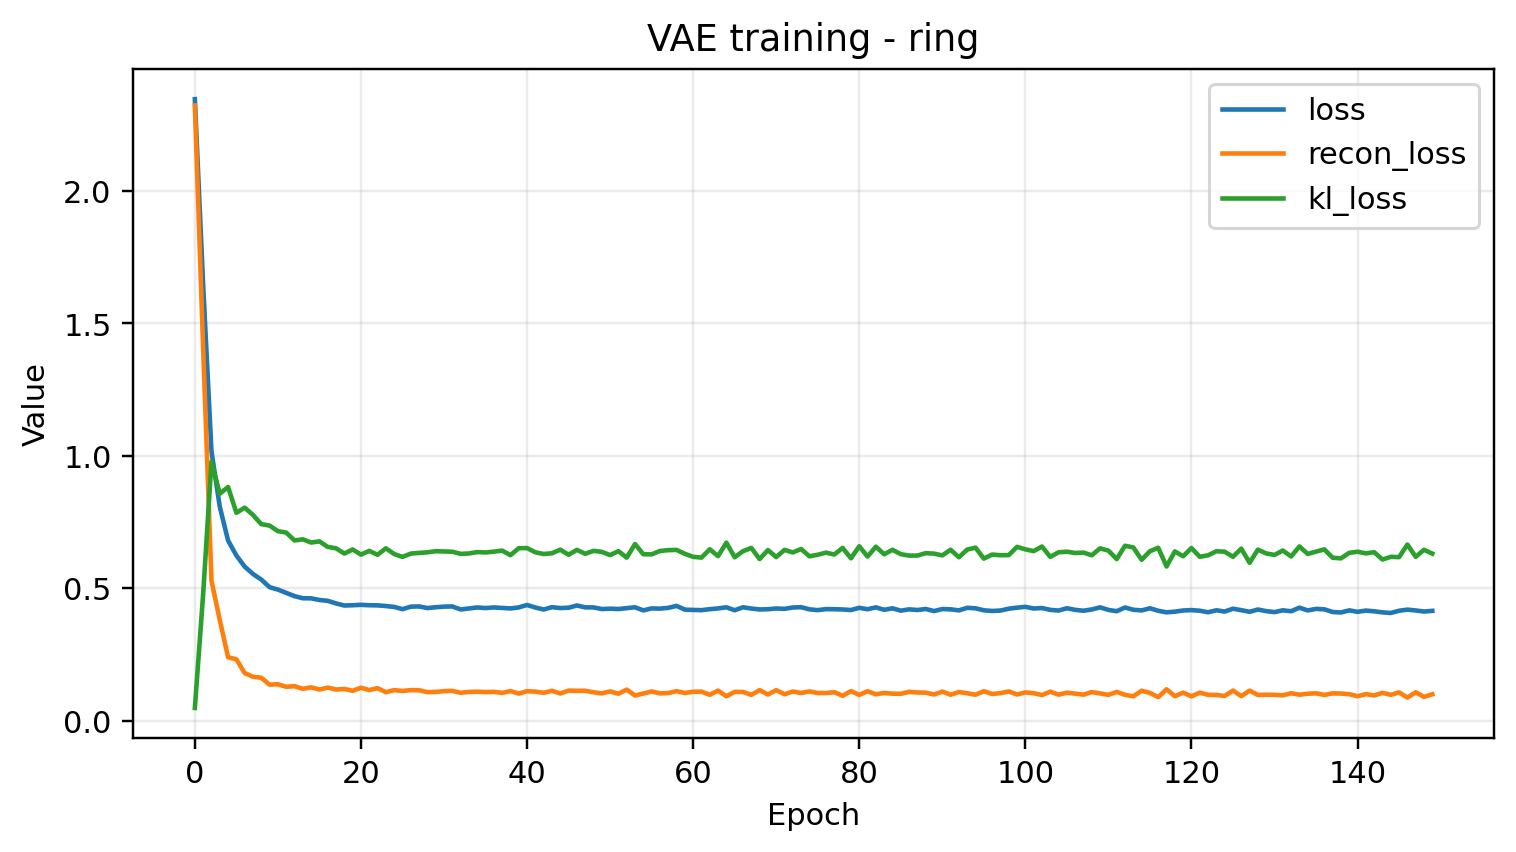
\includegraphics[width=\linewidth]{vae_ring_training.png}
    \caption{VAE on Ring}
\end{subfigure}
\hfill
\begin{subfigure}[b]{0.48\textwidth}
    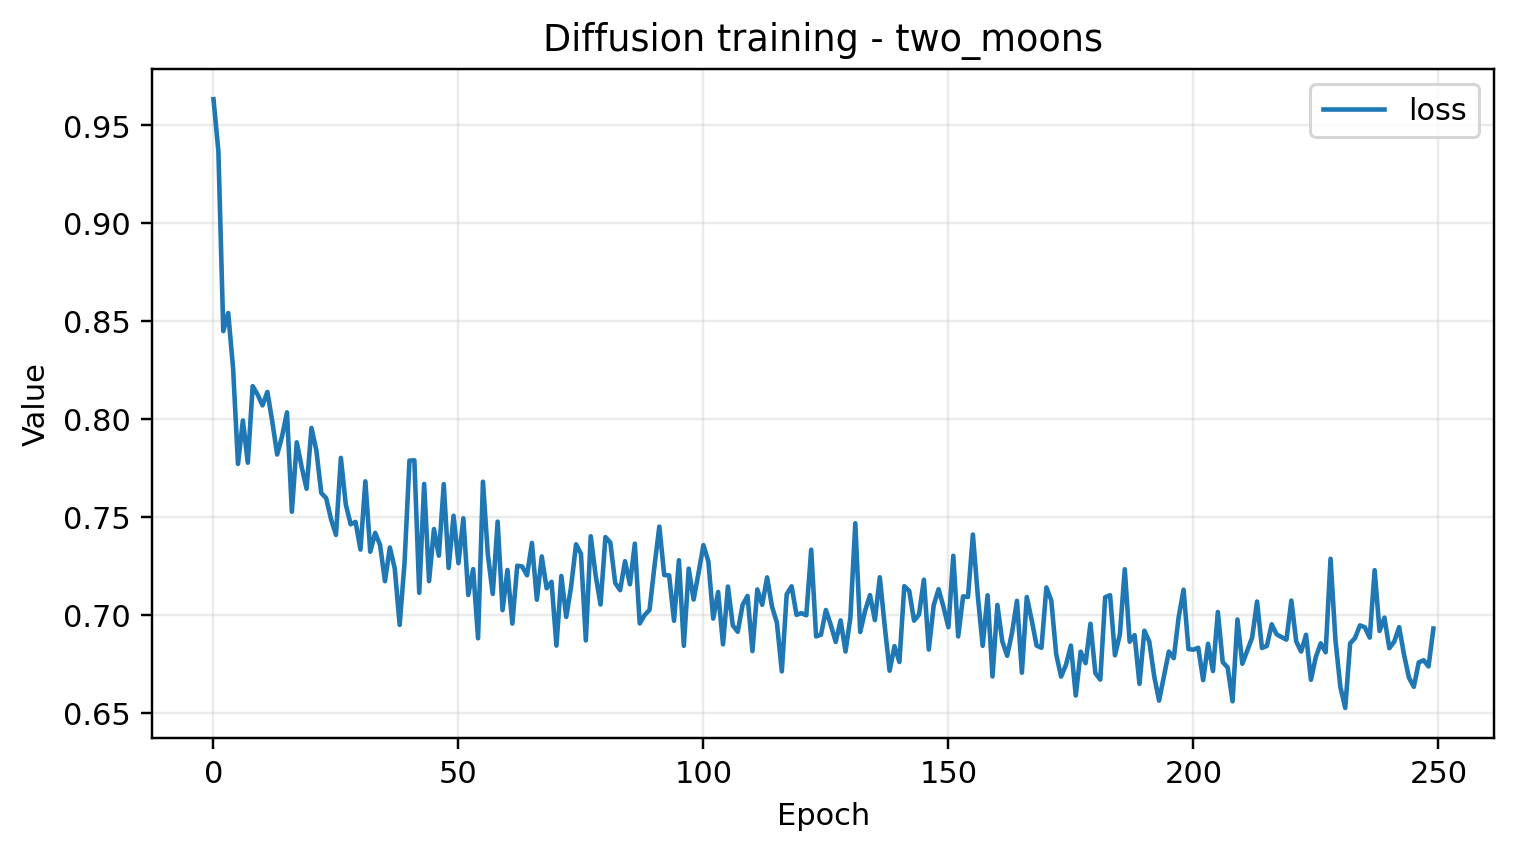
\includegraphics[width=\linewidth]{diffusion_two_moons_training.png}
    \caption{DDPM on Two Moons}
\end{subfigure}
\vspace{0.4em}
\begin{subfigure}[b]{0.48\textwidth}
    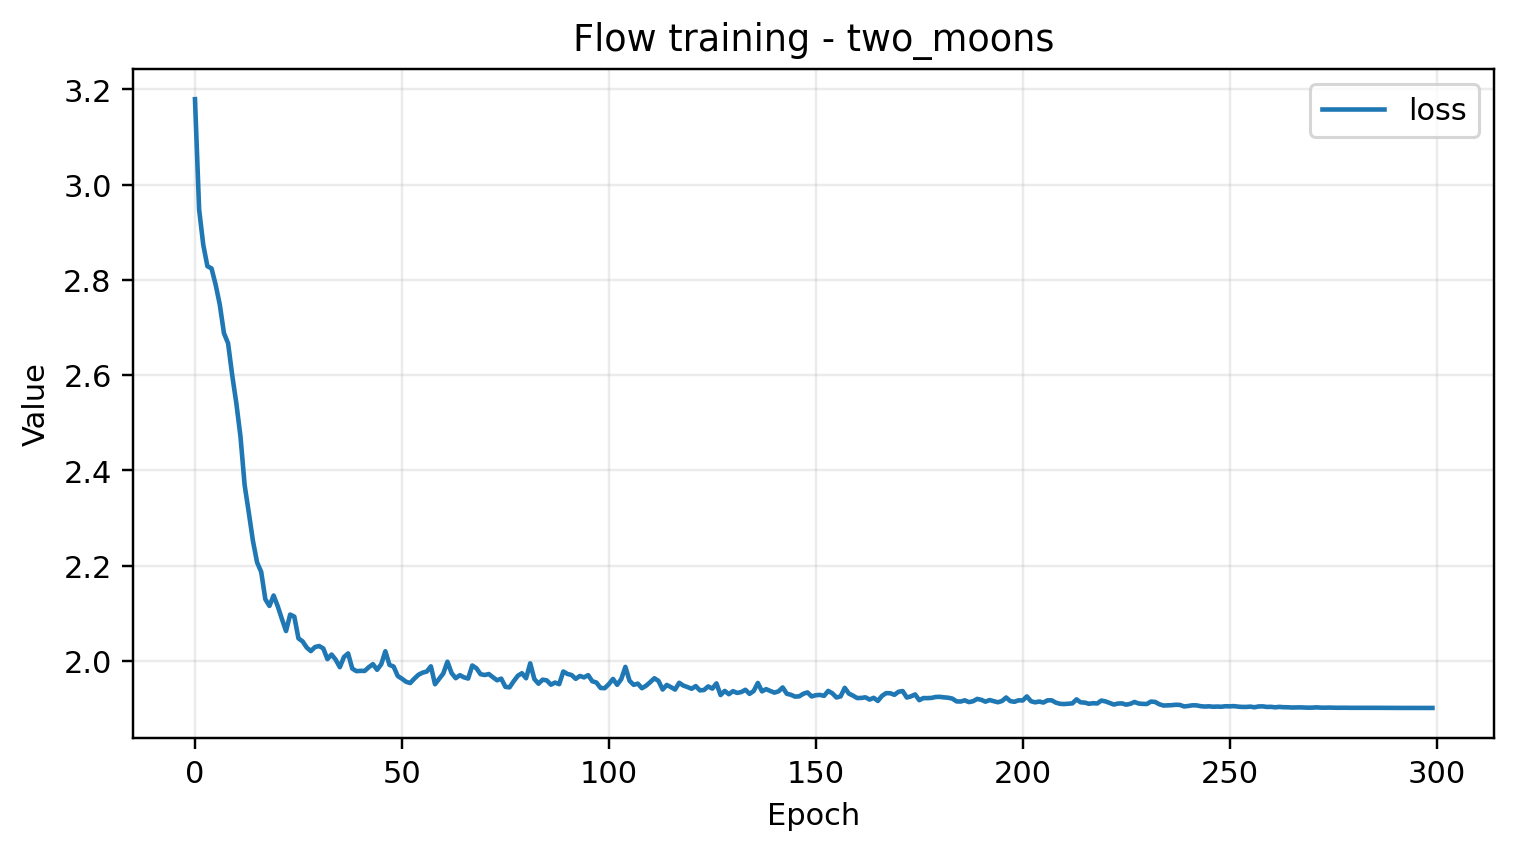
\includegraphics[width=\linewidth]{flow_two_moons_multiseed_s42_training.png}
    \caption{Flow on Two Moons}
\end{subfigure}
\hfill
\begin{subfigure}[b]{0.48\textwidth}
    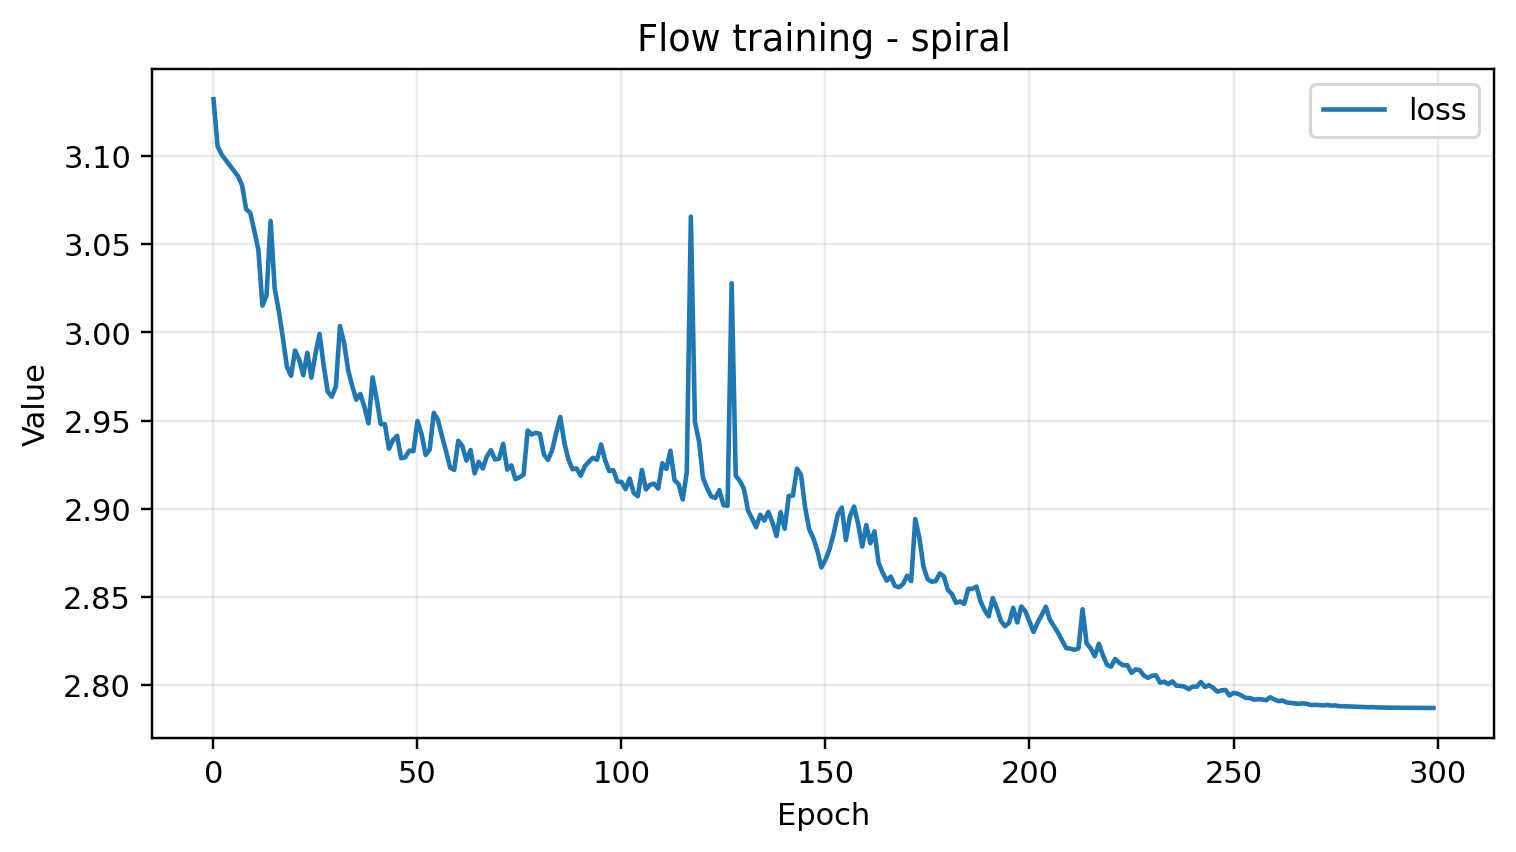
\includegraphics[width=\linewidth]{flow_spiral_multiseed_s42_training.png}
    \caption{Flow on Spiral}
\end{subfigure}
\caption{三类模型的代表性训练曲线。}
\end{figure}

从训练曲线来看，三类模型的收敛模式存在显著差异。VAE 的重构损失快速下降后趋于平稳，KL 项则先升后稳——这是典型的"先学结构、再规整潜空间"的训练动力学。DDPM 的噪声预测损失单调下降，但不同种子的收敛速度和最终水平波动较大（尤其在 Two Moons 上）。Flow 的负对数似然收敛最为缓慢但最为平稳：前 50 个 epoch 损失从约 3--5 快速下降到约 2，此后进入缓慢精调阶段，最终收敛到约 1.6--1.9（取决于数据集）。这种训练行为反映出精确似然优化的一个特点：收敛速度慢于近似目标，但一旦收敛则不会出现 ELBO 间隙或噪声预测误差带来的系统性偏差。

一个值得注意的现象是：Flow 在 Gaussian Mixture 上的部分种子（seed=42, 123）在修复缩放网络输出截断之前出现了 NaN 损失。仔细排查后发现，这些 NaN 是由仿射耦合层的 $\exp(s)$ 操作溢出了 float32 范围引起的。在缩放网络输出端加入 $\tanh$ 截断（乘以常数 3.0）后，所有种子都能稳定训练。这提醒我们：Flow 模型在数值稳定性上比 VAE 和 DDPM 更为敏感，合数范围控制是一个不可忽视的工程细节。

\subsection{生成样本可视化}

\begin{figure}[H]
\centering
\begin{subfigure}[b]{0.48\textwidth}
    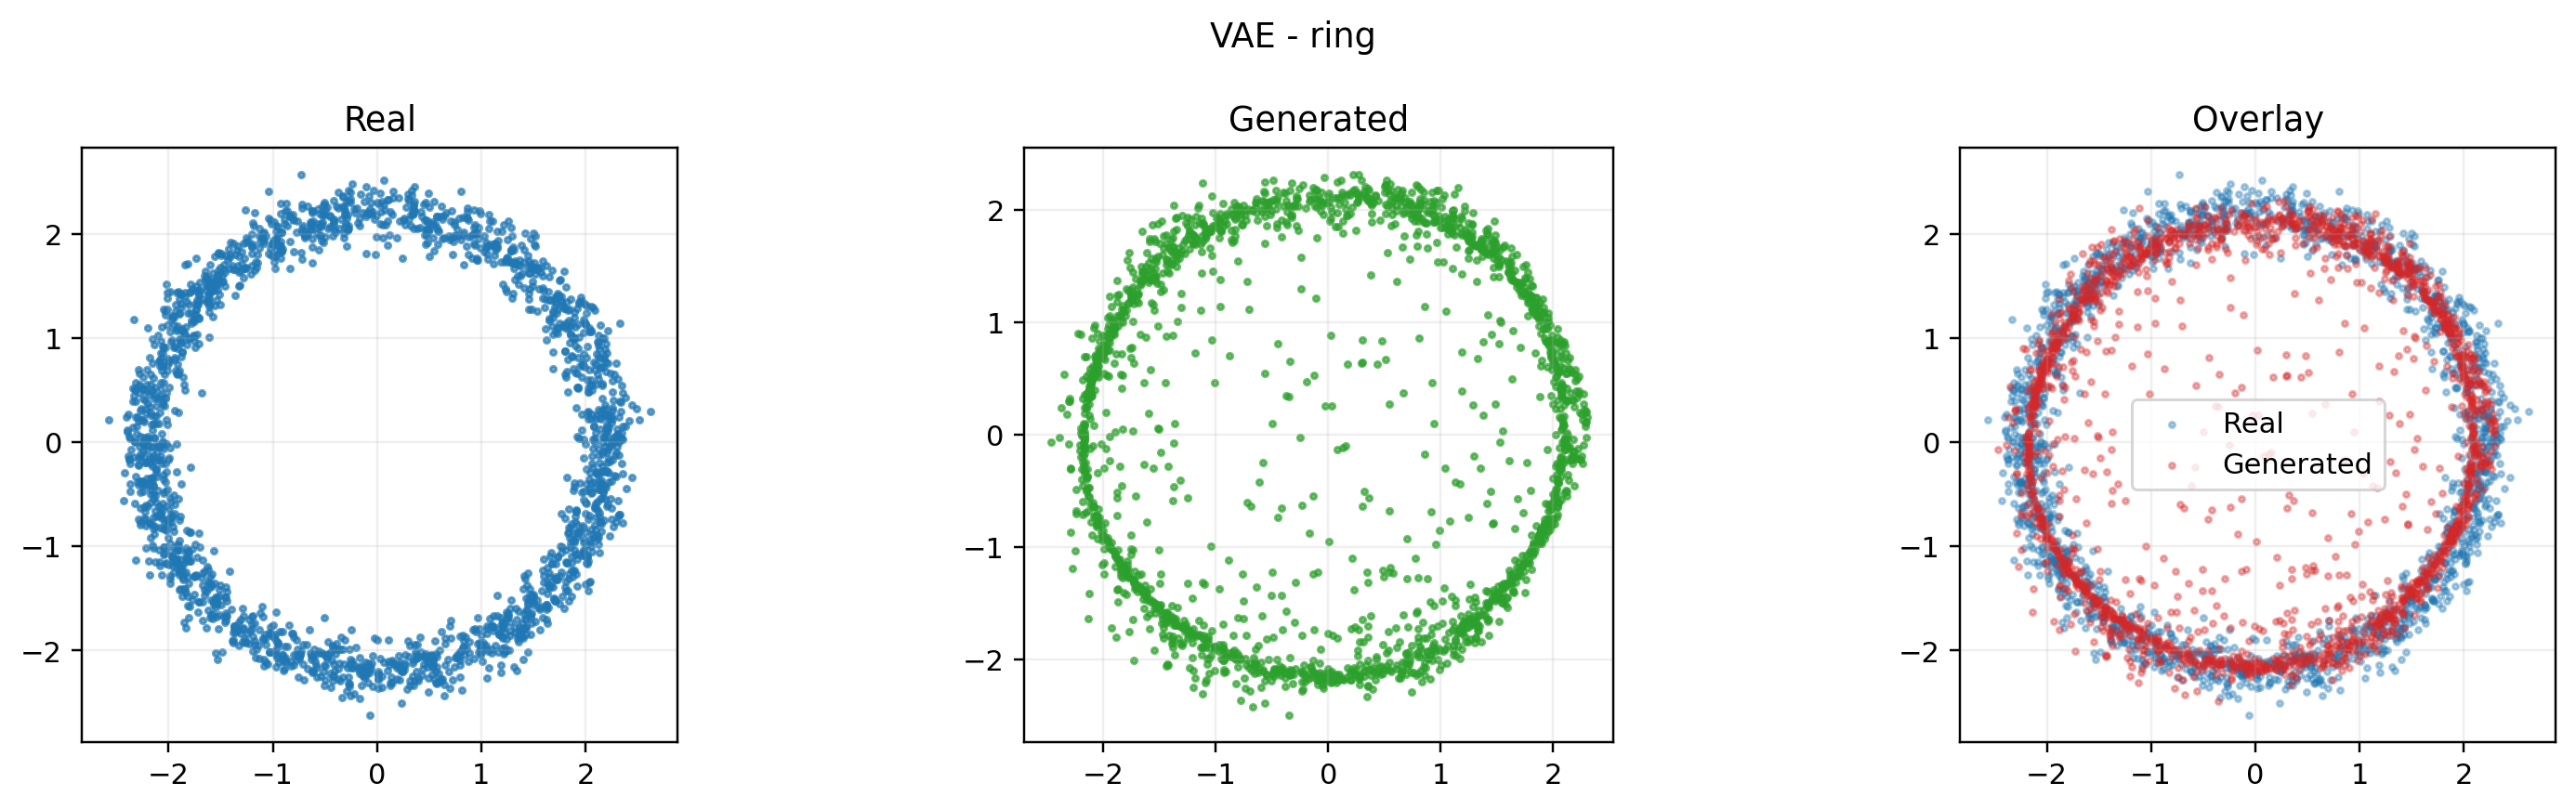
\includegraphics[width=\linewidth]{vae_ring_samples.png}
    \caption{VAE on Ring}
\end{subfigure}
\hfill
\begin{subfigure}[b]{0.48\textwidth}
    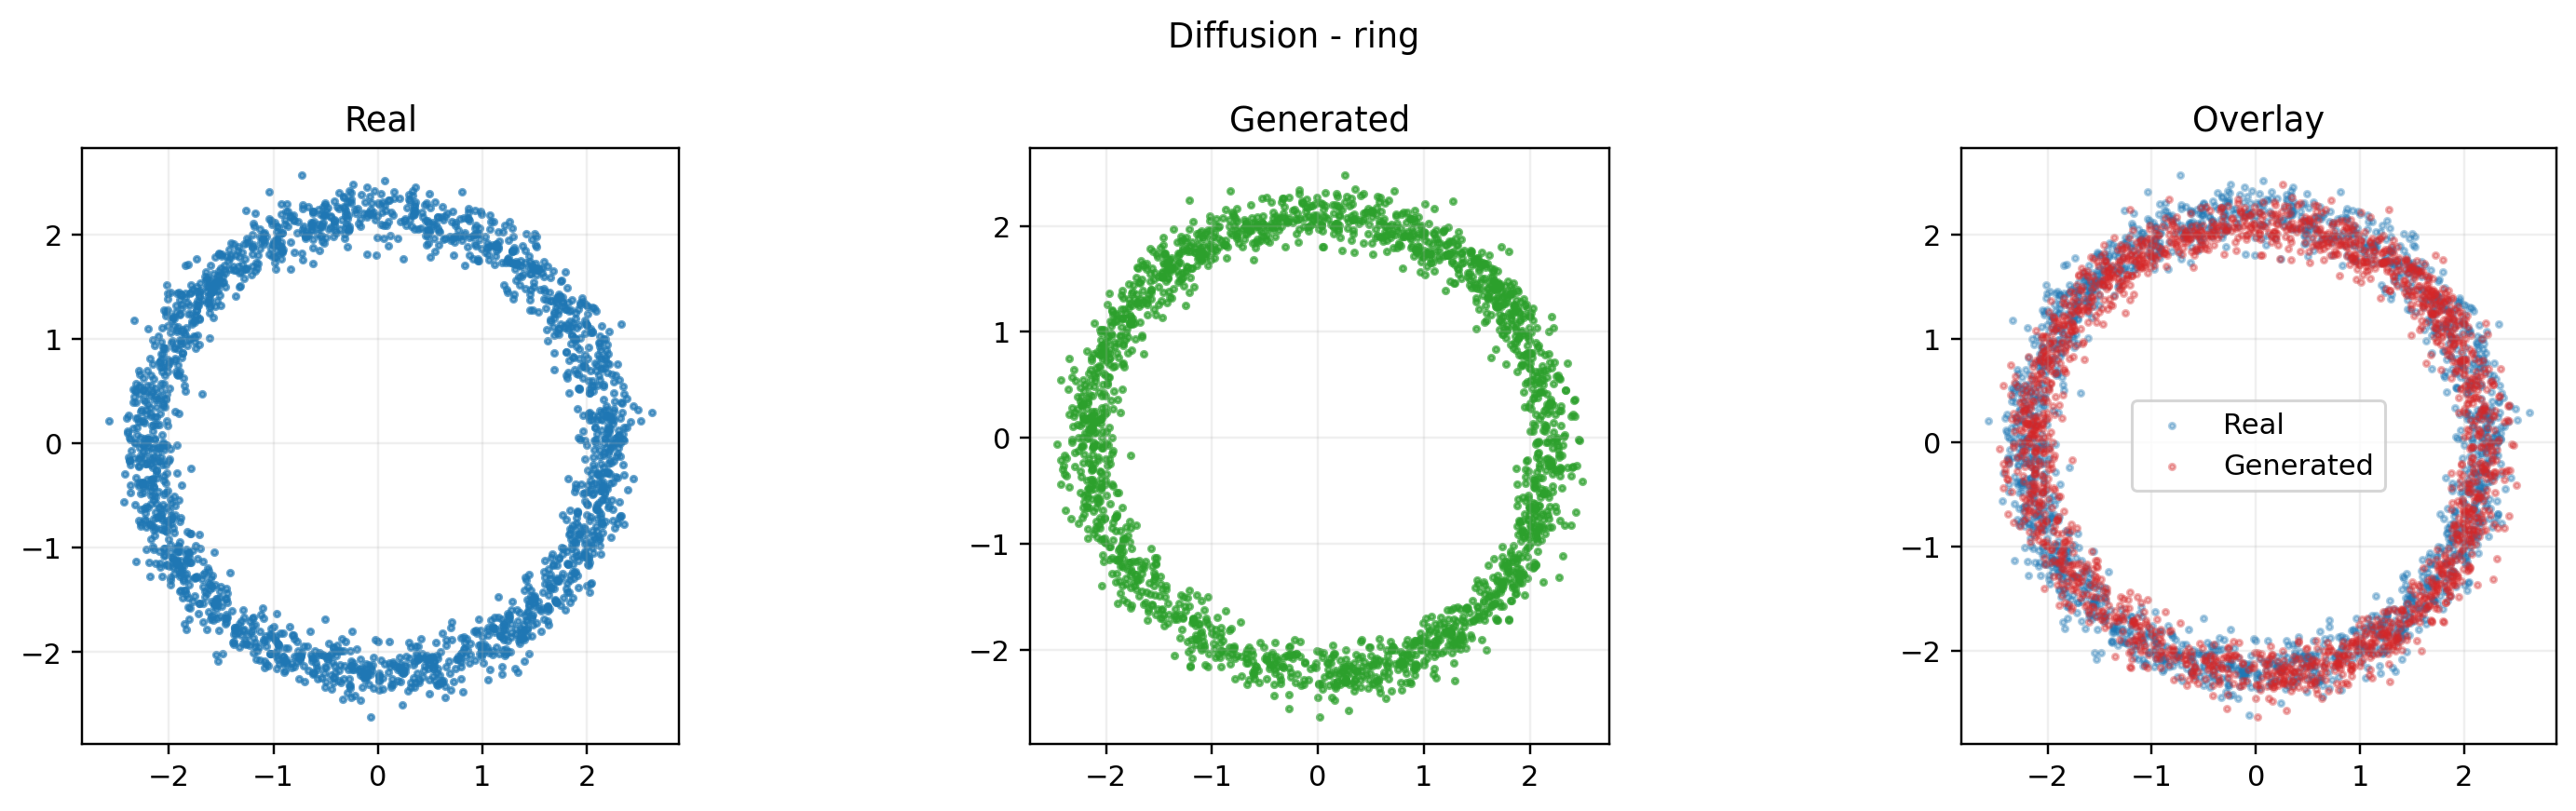
\includegraphics[width=\linewidth]{diffusion_ring_samples.png}
    \caption{DDPM on Ring}
\end{subfigure}
\vspace{0.4em}
\begin{subfigure}[b]{0.48\textwidth}
    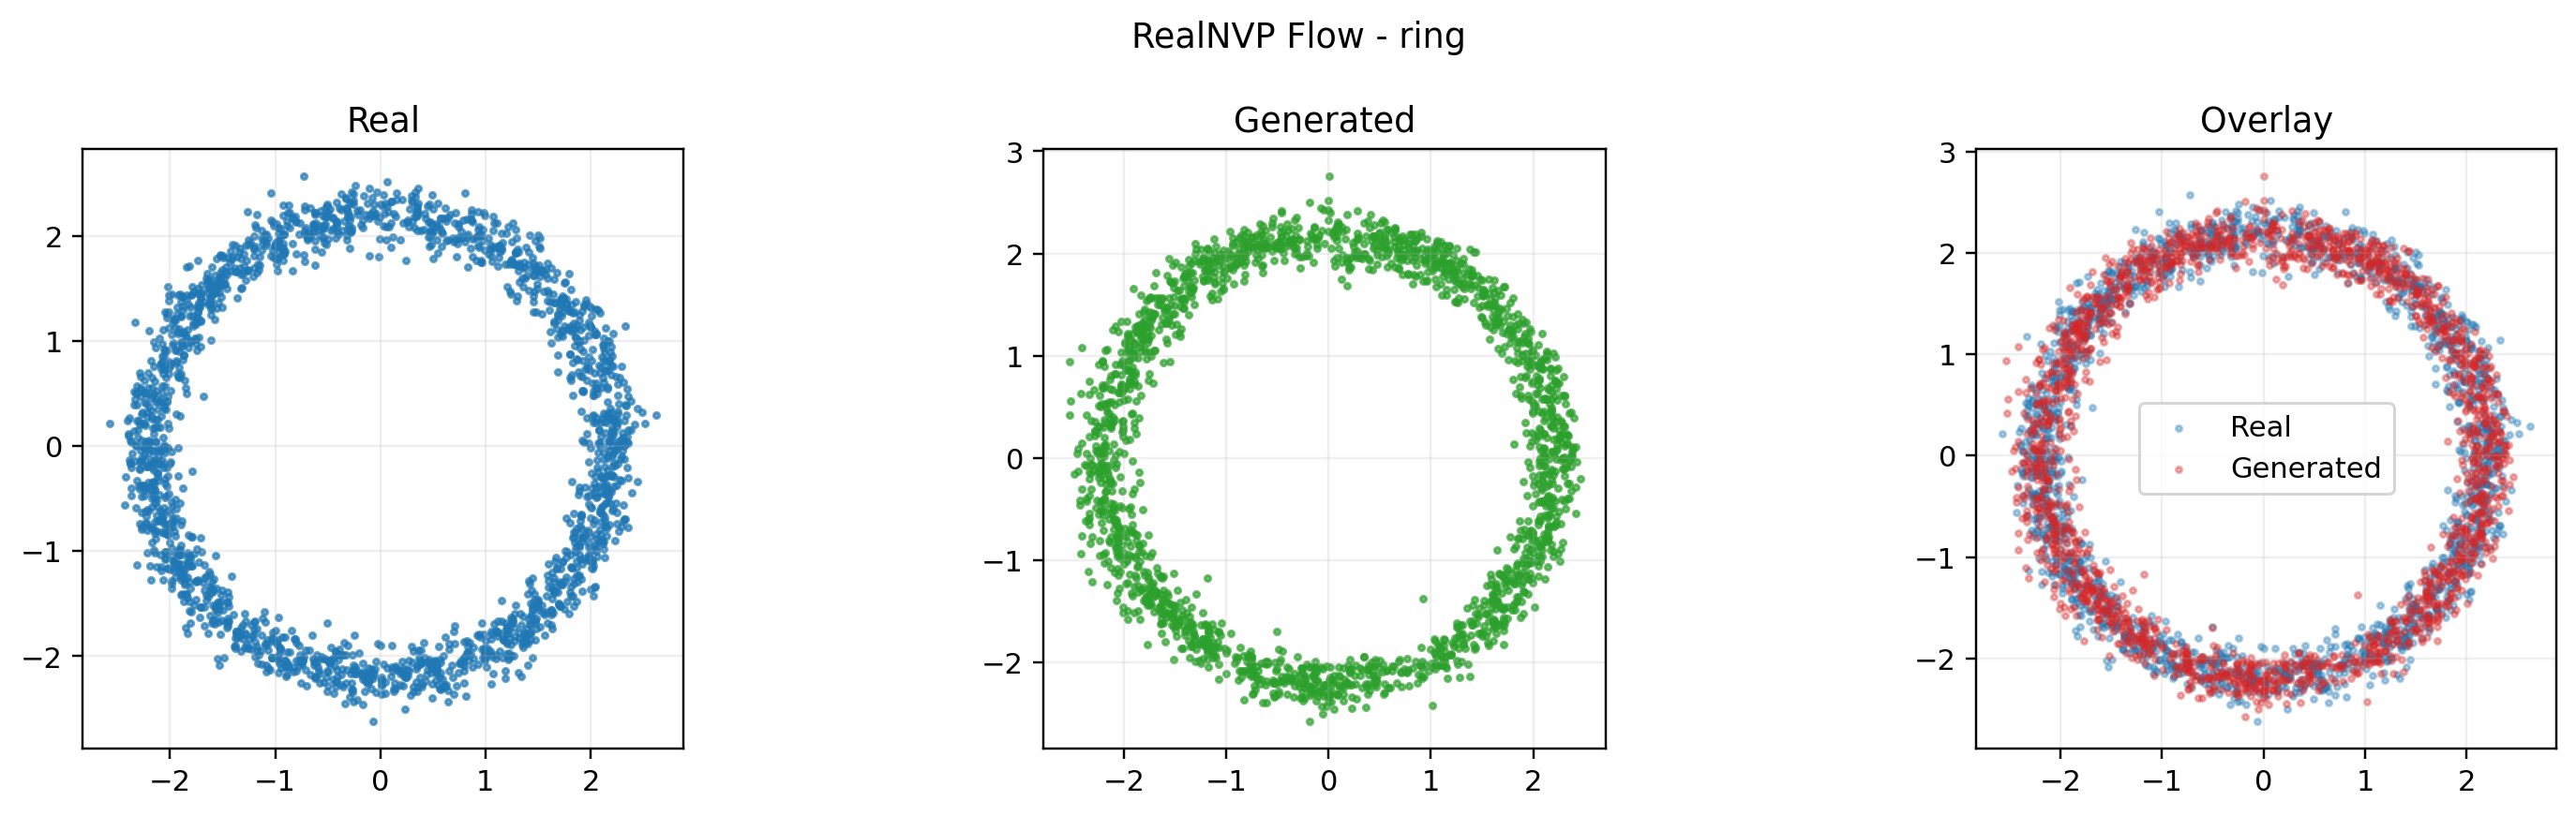
\includegraphics[width=\linewidth]{flow_ring_multiseed_s42_samples.png}
    \caption{Flow on Ring}
\end{subfigure}
\hfill
\begin{subfigure}[b]{0.32\textwidth}
    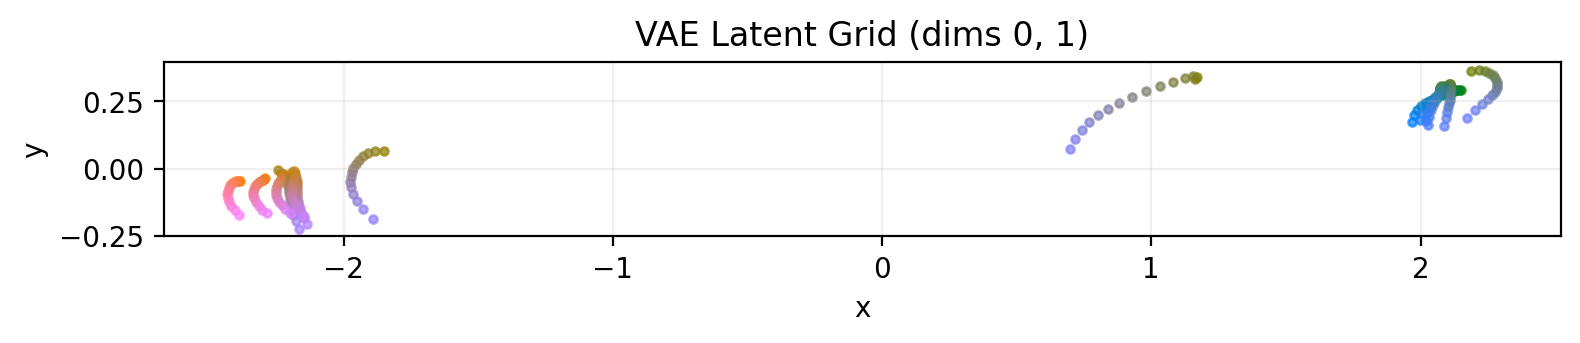
\includegraphics[width=\linewidth]{vae_ring_latent_grid.png}
    \caption{VAE 潜空间网格（Ring）}
\end{subfigure}
\caption{Ring 分布上的生成样本对比与 VAE 潜空间网格。}
\end{figure}

图~3 展示了 Ring 分布上的生成样本。定性观察与定量结论高度一致：VAE 倾向于将环带"涂厚"（生成点的径向散布明显大于真实数据），DDPM 能够较好地维持环状结构但个别区域厚度不均，Flow 生成的环带则最为清晰、均匀和最接近真实分布。这一可视化结果与 Flow 在 Ring 上三指标全优（MMD=$3.00\times10^{-4}$、SWD=$0.0512$、Chamfer=$0.0448$）的表现相互印证。

\begin{figure}[H]
\centering
\begin{subfigure}[b]{0.48\textwidth}
    
\includegraphics[width=\linewidth]{vae_spiral_samples.png}
    \caption{VAE on Spiral}
\end{subfigure}
\hfill
\begin{subfigure}[b]{0.48\textwidth}
    
\includegraphics[width=\linewidth]{diffusion_spiral_samples.png}
    \caption{DDPM on Spiral}
\end{subfigure}
\vspace{0.4em}
\begin{subfigure}[b]{0.48\textwidth}
    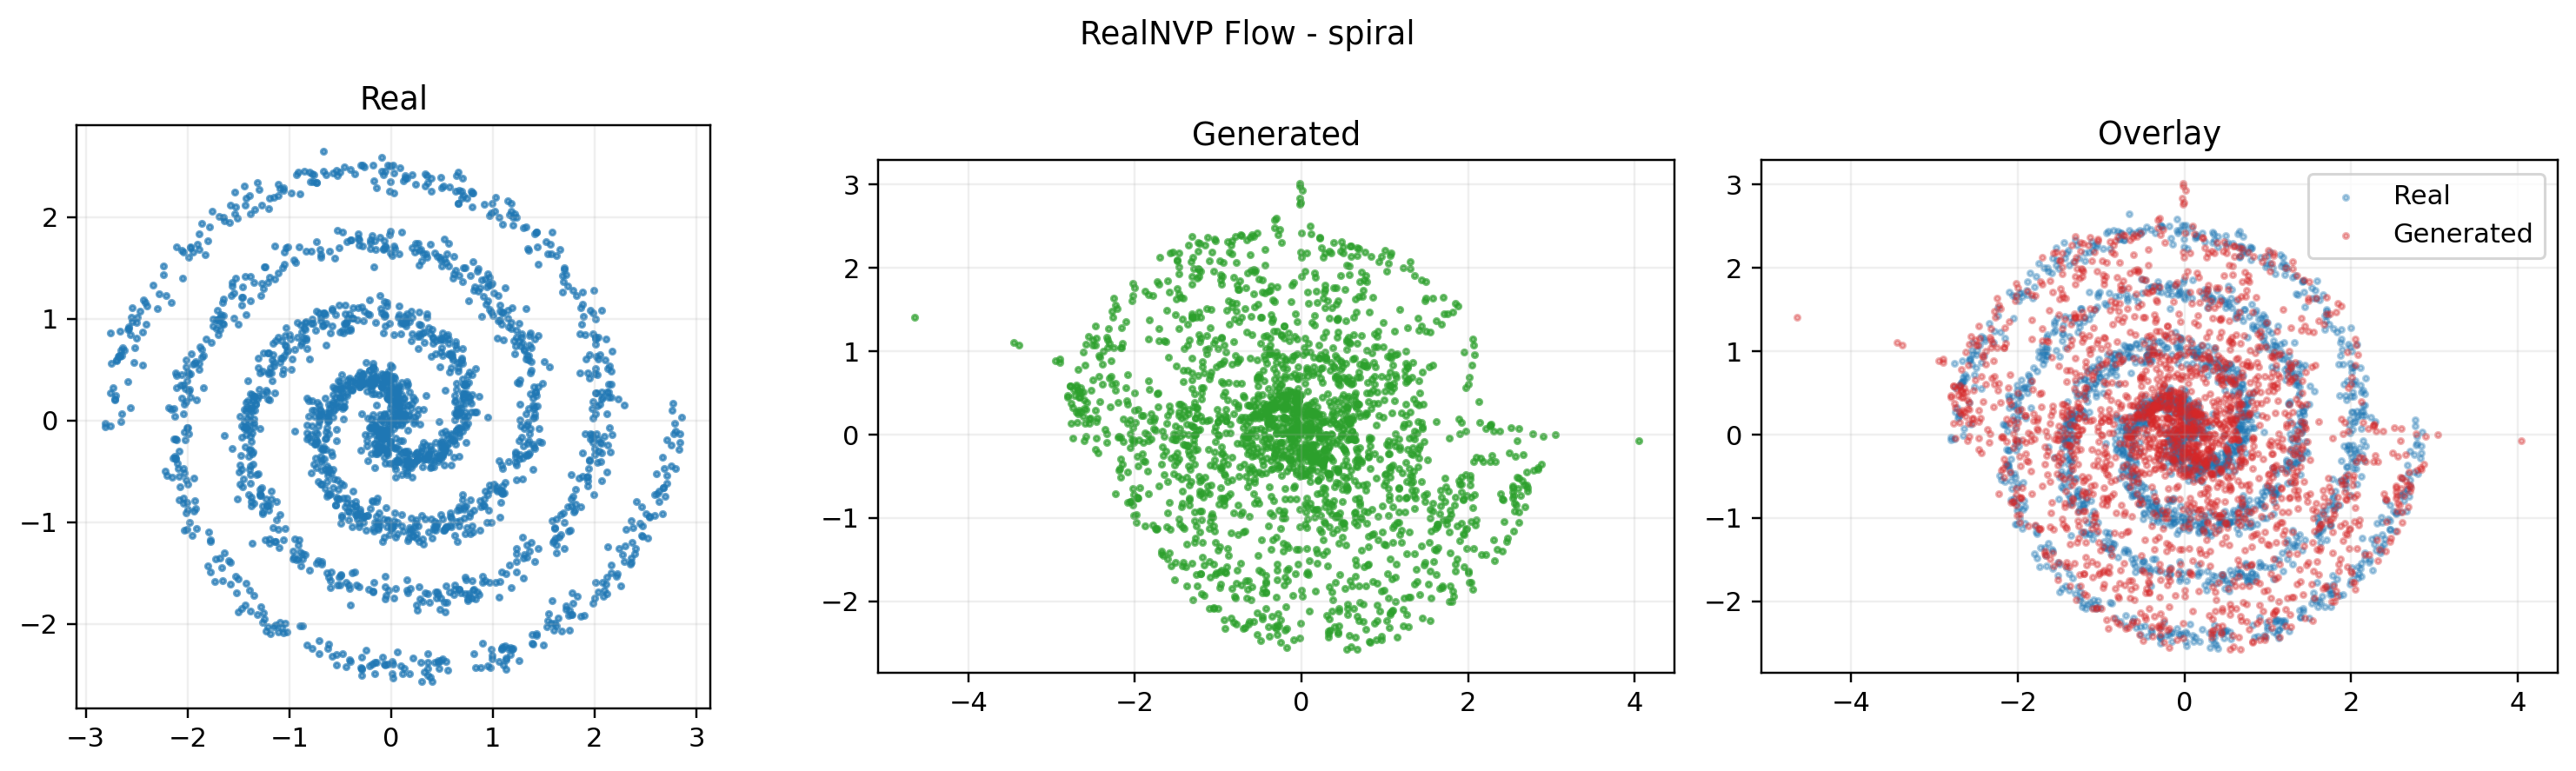
\includegraphics[width=\linewidth]{flow_spiral_multiseed_s42_samples.png}
    \caption{Flow on Spiral}
\end{subfigure}
\hfill
\begin{subfigure}[b]{0.32\textwidth}
    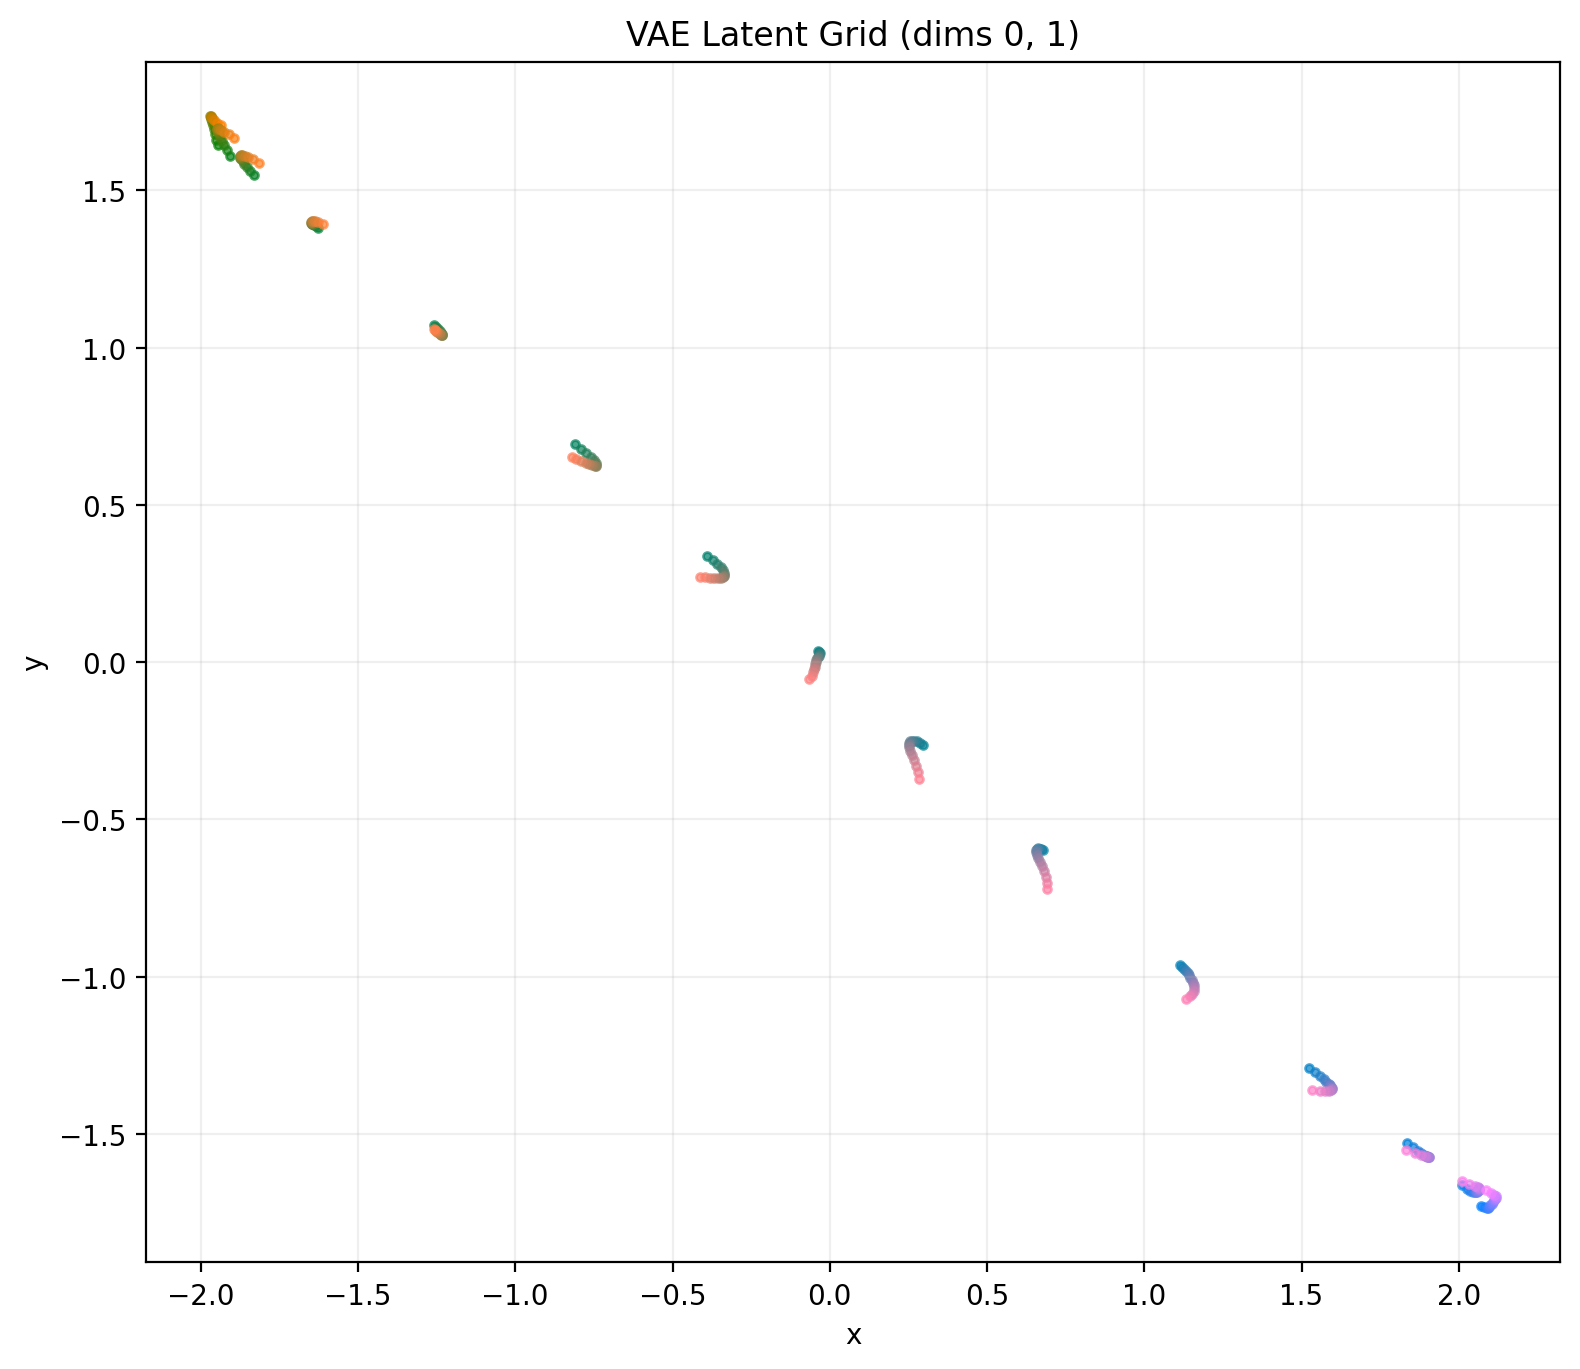
\includegraphics[width=\linewidth]{vae_spiral_latent_grid.png}
    \caption{VAE 潜空间网格（Spiral）}
\end{subfigure}
\caption{Spiral 分布上的生成样本对比与 VAE 潜空间网格。}
\end{figure}

在 Spiral 上，三类模型的差异更加鲜明。DDPM 生成的螺旋线在连续性和窄带上表现最好（与 MMD 略微领先的结论一致），但局部细节偶尔出现"断点"；Flow 生成的螺旋线在整体流畅性上接近 DDPM，但某些局部区域的宽度略偏大；VAE 则明显平滑化了螺旋线，尤其是在臂的末端区域出现了断裂和过度平滑。这些可视化结果清楚地说明：对于长程连续拓扑结构，分步去噪机制确实比单步解码或可逆映射具有内禀的优势。

\subsection{潜空间结构分析}

VAE 的一个独特优势是其显式的低维潜空间具有可解释性。图~3(d) 和图~4(d) 展示了通过在潜空间两个主导维度上做均匀网格采样再解码得到的结果。从图中可以清楚地看到，潜空间在 Ring 分布上学到的是"以原点为中心向外辐射"的结构，而在 Spiral 分布上学到的则是更复杂的非线性扭曲结构。这种可视化不仅帮助理解 VAE 学到了什么，也揭示了其局限性：当数据分布具有复杂的全局拓扑（如螺旋）时，2D 潜空间的表达能力明显不足，需要更多维度（本文使用 $d=4$）才能将结构"展开"。

潜空间插值实验（见附录）进一步展示了 VAE 在潜空间中连续变化的平滑性，这也从侧面验证了 KL 正则项确实起到了规整潜空间的作用。

\subsection{扩散去噪过程可视化}

\begin{figure}[H]
\centering

\includegraphics[width=0.95\textwidth]{diffusion_ring_enhanced_snapshots.png}
\caption{DDPM 在 Ring 上的十步去噪过程快照（$T=80$）。从左到右、从上到下：纯噪声逐步恢复为清晰环带。}
\end{figure}

图~5 展示了 DDPM 从纯噪声逐步"雕刻"出环状结构的完整过程。可以看到，在 $t\approx 79$（早期阶段）样本几乎完全是各向同性的高斯噪声；到 $t\approx 52$ 时开始出现模糊的圆形轮廓；到 $t\approx 26$ 时环带结构已经比较清晰；最终 $t=0$ 时收敛为细薄的闭合环带。这种"从无序到有序"的渐进生成过程是扩散模型最核心的特征，也是它在复杂几何结构上保持优势的根本原因。

与 VAE 的单步生成和 Flow 的一步逆变换不同，DDPM 将复杂的全局生成任务分解为约 80 个局部去噪子任务。每一步只负责将当前带噪样本向数据流形"挪动一小步"，这使得每一步的学习难度都远小于直接生成。当然，代价也很直接——采样需要执行全部 80 次前向推理。

\subsection{综合对比与范式讨论}

将上述定性和定量结果放在一起，可以对三类生成范式的适用边界做出以下判断。

\textbf{在分布质量方面，}RealNVP 凭借精确的似然优化，在 Gaussian Mixture、Ring 和 Two Moons 三个分布上都取得了最优的 MMD，且在 Ring 和 Two Moons 上实现了三项核心指标的全优。这背后的原因在于：Flow 模型不引入变分间隙（VAE 的局限）也不需要离散化近似（DDPM 的局限），在模型容量充足时能够原则上精确地恢复任意分布。唯一的例外是 Spiral，DDPM 在 MMD 上微弱领先，说明对于极端复杂的长程拓扑结构，分步去噪的"分而治之"策略仍然具有不可替代的优势。

\textbf{在局部几何精度方面，}DDPM 的平均 Chamfer 距离（0.0578）在全局最优，体现了其逐步去噪机制在处理局部邻域贴合上的优势。Flow 的平均 Chamfer（0.0628）与 DDPM 差距不大，说明可逆变换在局部几何上也具备相当的竞争力。VAE 的平均 Chamfer（0.0830）则明显偏大，这是单步解码导致的平滑化效应。

\textbf{在采样效率方面，}VAE 以平均 $0.6$\,ms 的采样时间一骑绝尘，Flow 以约 $2.3$\,ms 紧随其后，DDPM 则需要约 $14.7$\,ms——是 Flow 的约 6.4 倍、VAE 的约 25 倍。在大规模生成任务的场景下，这一差距可能成为工程选型的关键考量。

\textbf{在训练稳定性方面，}VAE 和 DDPM 都非常稳健，五种子结果的标准差较小，未见 NaN 或训练崩溃；而 Flow 在早期的实验中出现了 NaN 损失（因缩放网络输出溢出），需要额外的数值截断技巧才能稳定。这是一个在实践中不可忽视的工程性问题。

% ===================== 五、误差分析与局限性 =====================
\section{误差分析、权衡与局限性}

任何比较研究都有其边界条件。本节从方法论和实验结果两个角度分析本文的设计局限和潜在的误差来源。

\subsection{各模型的内在误差来源}

\textbf{VAE 的误差来源：}ELBO 本质上只是对数似然的一个下界，下界和真实似然之间的差距（即变分间隙）无法从 ELBO 本身直接估计。当数据分布具有极薄的结构（如 Ring 的窄环带或 Spiral 的细螺旋线）时，编码器需要将连续流形上的点映射到紧致的潜空间区域，这会导致较大的重构误差。此外，对角高斯后验的假设限制了编码器表达复杂后验分布的能力。这些因素共同导致了 VAE 在 Ring 和 Spiral 上的较差表现。

\textbf{DDPM 的误差来源：}DDPM 最根本的局限来自离散化。虽然理论上当 $T\to\infty$ 且步长趋于零时扩散过程可以精确地恢复任意分布，但在实践中 $T=80$ 的有限步数引入了一定的离散化误差，尤其是在低密度区域和分布边界处。此外，DDPM 的优化目标只是一个等效的噪声预测 MSE，而不是直接的对数似然，因此最优的噪声预测器并不严格对应最优的生成模型。Two Moons 上 DDPM 的高方差表现（跨种子的 MMD 标准差 $1.39\times10^{-3}$）很可能就是这种等效优化带来的间接后果——噪声预测 MSE 的细微差异在复杂的局部拓扑上被放大了。

\textbf{RealNVP 的误差来源：}Flow 模型的精确似然性质建立在所有耦合层严格可逆且雅可比行列式计算精确的假设之上。然而，$\tanh$ 截断虽然解决了数值稳定性问题，但也限制了缩放网络的动态范围（$\exp(s)\in[e^{-3},e^{3}]$），这意味着某些需要极端缩放或压缩的几何变换无法被完美表达。此外，耦合层架构的三角雅可比结构虽然高效，但也限制了每一层只能变换一半的维度，需要更多的层数来补偿。在 Spiral 这种极端拓扑上，8 层耦合层可能仍然不足以完全展开螺旋结构，这是 Flow 在 Spiral MMD 上未能超越 DDPM 的一个可能原因。

\subsection{实验设计的局限性}

\begin{enumerate}
    \item \textbf{网络容量的可比性：} 虽然本文统一了隐藏维度和深度，但三类模型的有效参数量并不严格相等：Flow 的 8 层耦合层（每层包含两个独立网络）的参数量大约是 VAE 的 4--5 倍。这在"公平比较"和"让各类模型发挥最佳性能"之间存在张力。本文倾向于后者，因为如果强行用参数最少的 VAE 限制其他模型的容量，反而会让比较失去实际参考价值。

    \item \textbf{超参数搜索的有限性：} 本文对各类模型仅采用了单一的推荐超参数配置，没有做网格搜索或贝叶斯优化。例如，DDPM 的扩散步数 $T$ 和 VAE 的 $\beta$ 权重都可能通过进一步的调参获得更好的结果。Flow 的耦合层数 $K$ 和截断系数 $3.0$ 同样有优化空间。

    \item \textbf{评价指标的局限性：} 虽然本文使用了六种互补指标，但每种指标都只能反映生成质量的某一侧面。MMD 对核函数和带宽敏感；SWD 受投影方向数量的影响；Chamfer 距离无法区分"生成点都聚在一个真实点附近"和"均匀覆盖但有微小偏移"这两种本质上不同的行为。GMM-NLL 和 KDE-NLL 作为似然代理指标，其结果依赖于高斯混合模型的分量数或核密度的带宽选择。

    \item \textbf{二维场景的泛化性：} 本文的所有结论都建立在对二维分布的实验之上。高维场景下，Flow 的计算代价将随维度增加而增长（耦合层需要更多的层数和更宽的网络），DDPM 的采样成本也将显著上升，VAE 则可能因为潜空间的维度诅咒而面临新的挑战。二维结论向高维的外推需要谨慎。

    \item \textbf{模型的实现质量：} 本文中三类模型的骨干网络都是基于 MLP 的简单实现，没有引入 Batch Normalization、自注意力或更高级的架构组件。更精细的网络设计可能会改变三类模型的相对排序。
\end{enumerate}

% ===================== 六、总结与展望 =====================
\section{总结与展望}

\subsection{主要结论}

本文围绕二维分布生成建模这一主题，在统一实验框架下系统比较了 VAE、DDPM 和 RealNVP 三类代表性深度生成模型，得到以下主要结论：

\begin{enumerate}
    \item \textbf{RealNVP 在分布拟合质量上整体最优。}在全部四个分布上的平均 MMD 为 $4.73\times10^{-4}$，比 VAE 低 3.2 倍，比 DDPM 低 3.8 倍；在 Ring 和 Two Moons 上更是取得了 MMD、SWD、Chamfer 三项核心指标的全优。这说明精确似然优化在低维生成任务中具有明显的理论优势。

    \item \textbf{DDPM 在局部几何精度上保持领先，且在极端复杂拓扑上不可替代。}DDPM 的平均 Chamfer 距离为 0.0578，是三者中最优的；在 Spiral 上的 MMD 也以微弱优势领先 Flow。分步去噪机制对于长程连续拓扑结构具有内禀的优势，这种优势在更复杂的几何上可能会进一步放大。

    \item \textbf{VAE 在采样速度上保持绝对优势}（平均 0.6\,ms），但在生成质量上整体落后。潜空间可视化表明，VAE 的局限主要来自单步解码带来的平滑化效应和对角高斯后验的表达能力限制。

    \item \textbf{三类模型形成了清晰的"精度—速度"谱系：}VAE 最快但最粗糙，DDPM 最精细但最慢，Flow 在精度上接近甚至超过 DDPM 的同时保持了接近 VAE 的采样速度，构成了一个相当有吸引力的折中方案。
\end{enumerate}

\subsection{展望}

基于本文的工作，有几个方向值得进一步探索。首先，将 Latent Diffusion（在 VAE 潜空间中做扩散）与 Flow 结合起来——用 VAE 压缩维度后再用 Flow 建模潜空间分布——可能在高维场景中同时获得三类范式的优势。其次，本文的所有实验都在二维分布上进行，将同样的比较框架扩展到更高维度（如 8 维 lifted 数据或小型图像数据集）将进一步检验结论的泛化性。最后，引入更现代的生成模型变体（如基于连续时间 SDE 的扩散模型、带有自注意力机制的 Flow 架构）将有助于判断本文结论在多大程度上来自生成范式本身，在多大程度上来自具体的实现选择。

% ===================== 附录 =====================
\appendix
\section{补充图表}

\begin{figure}[H]
\centering
\begin{subfigure}[b]{0.48\textwidth}
    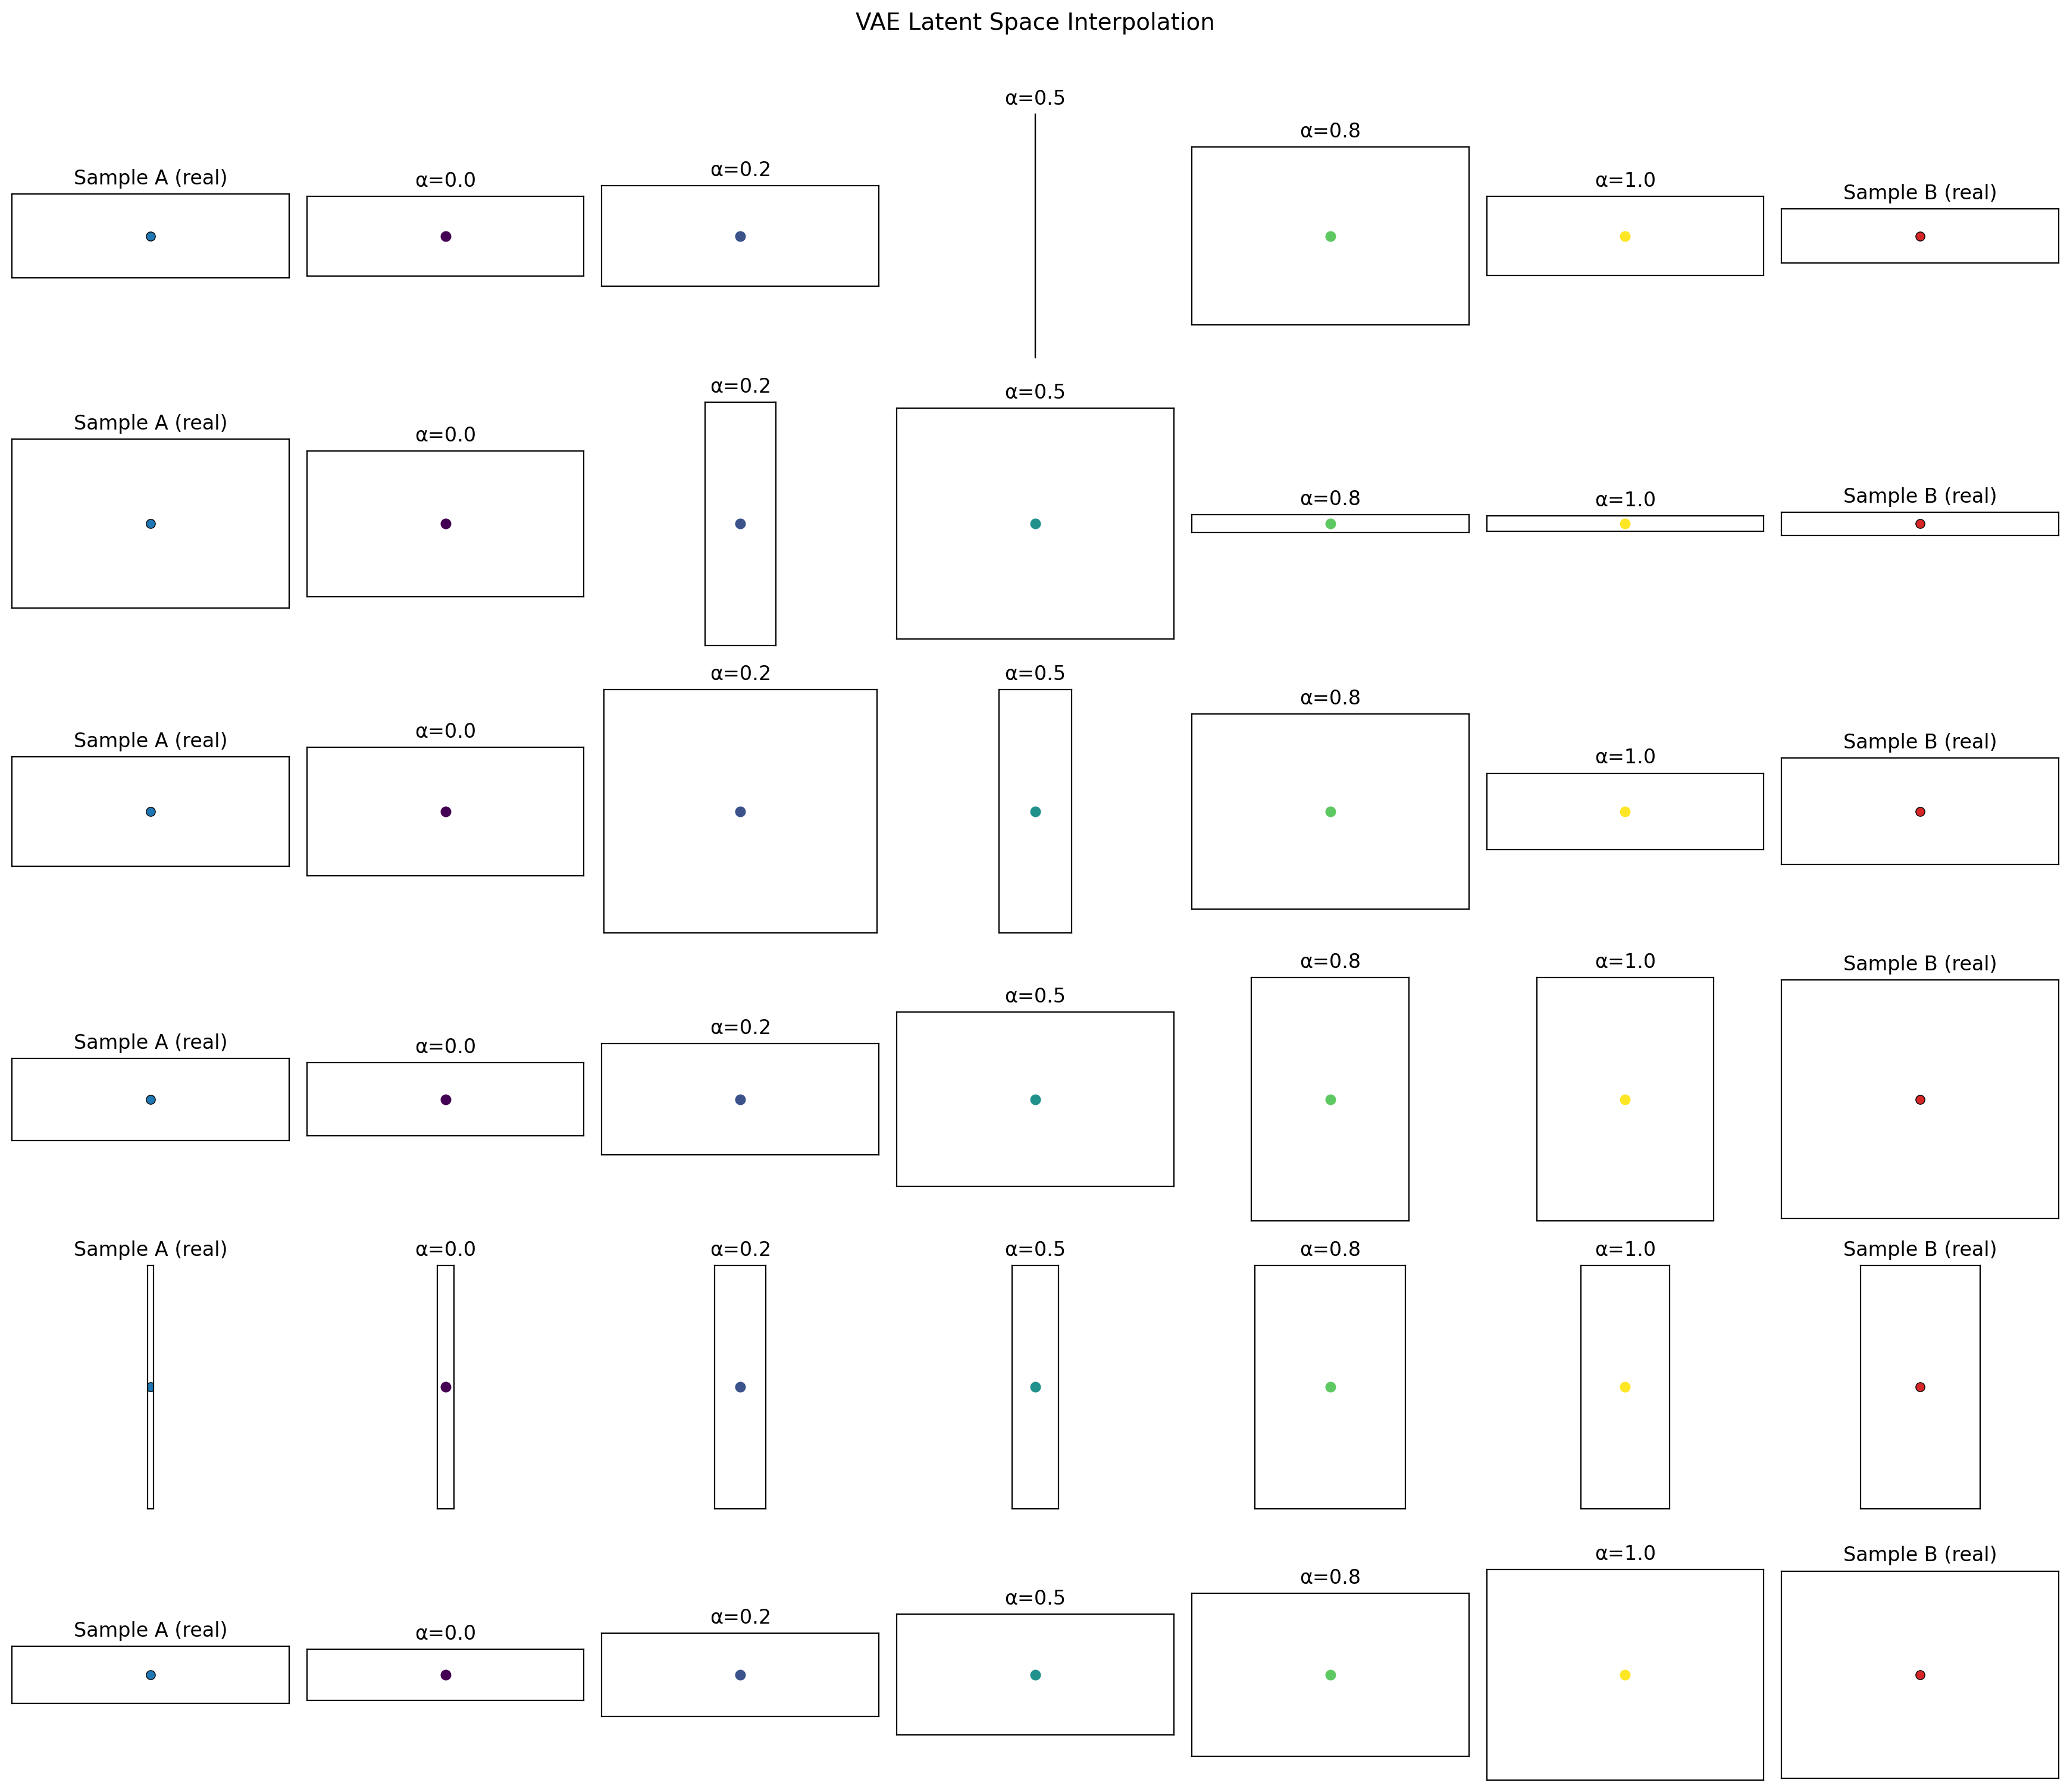
\includegraphics[width=\linewidth]{vae_two_moons_latent_interpolation.png}
    \caption{VAE on Two Moons: 潜空间插值}
\end{subfigure}
\hfill
\begin{subfigure}[b]{0.48\textwidth}
    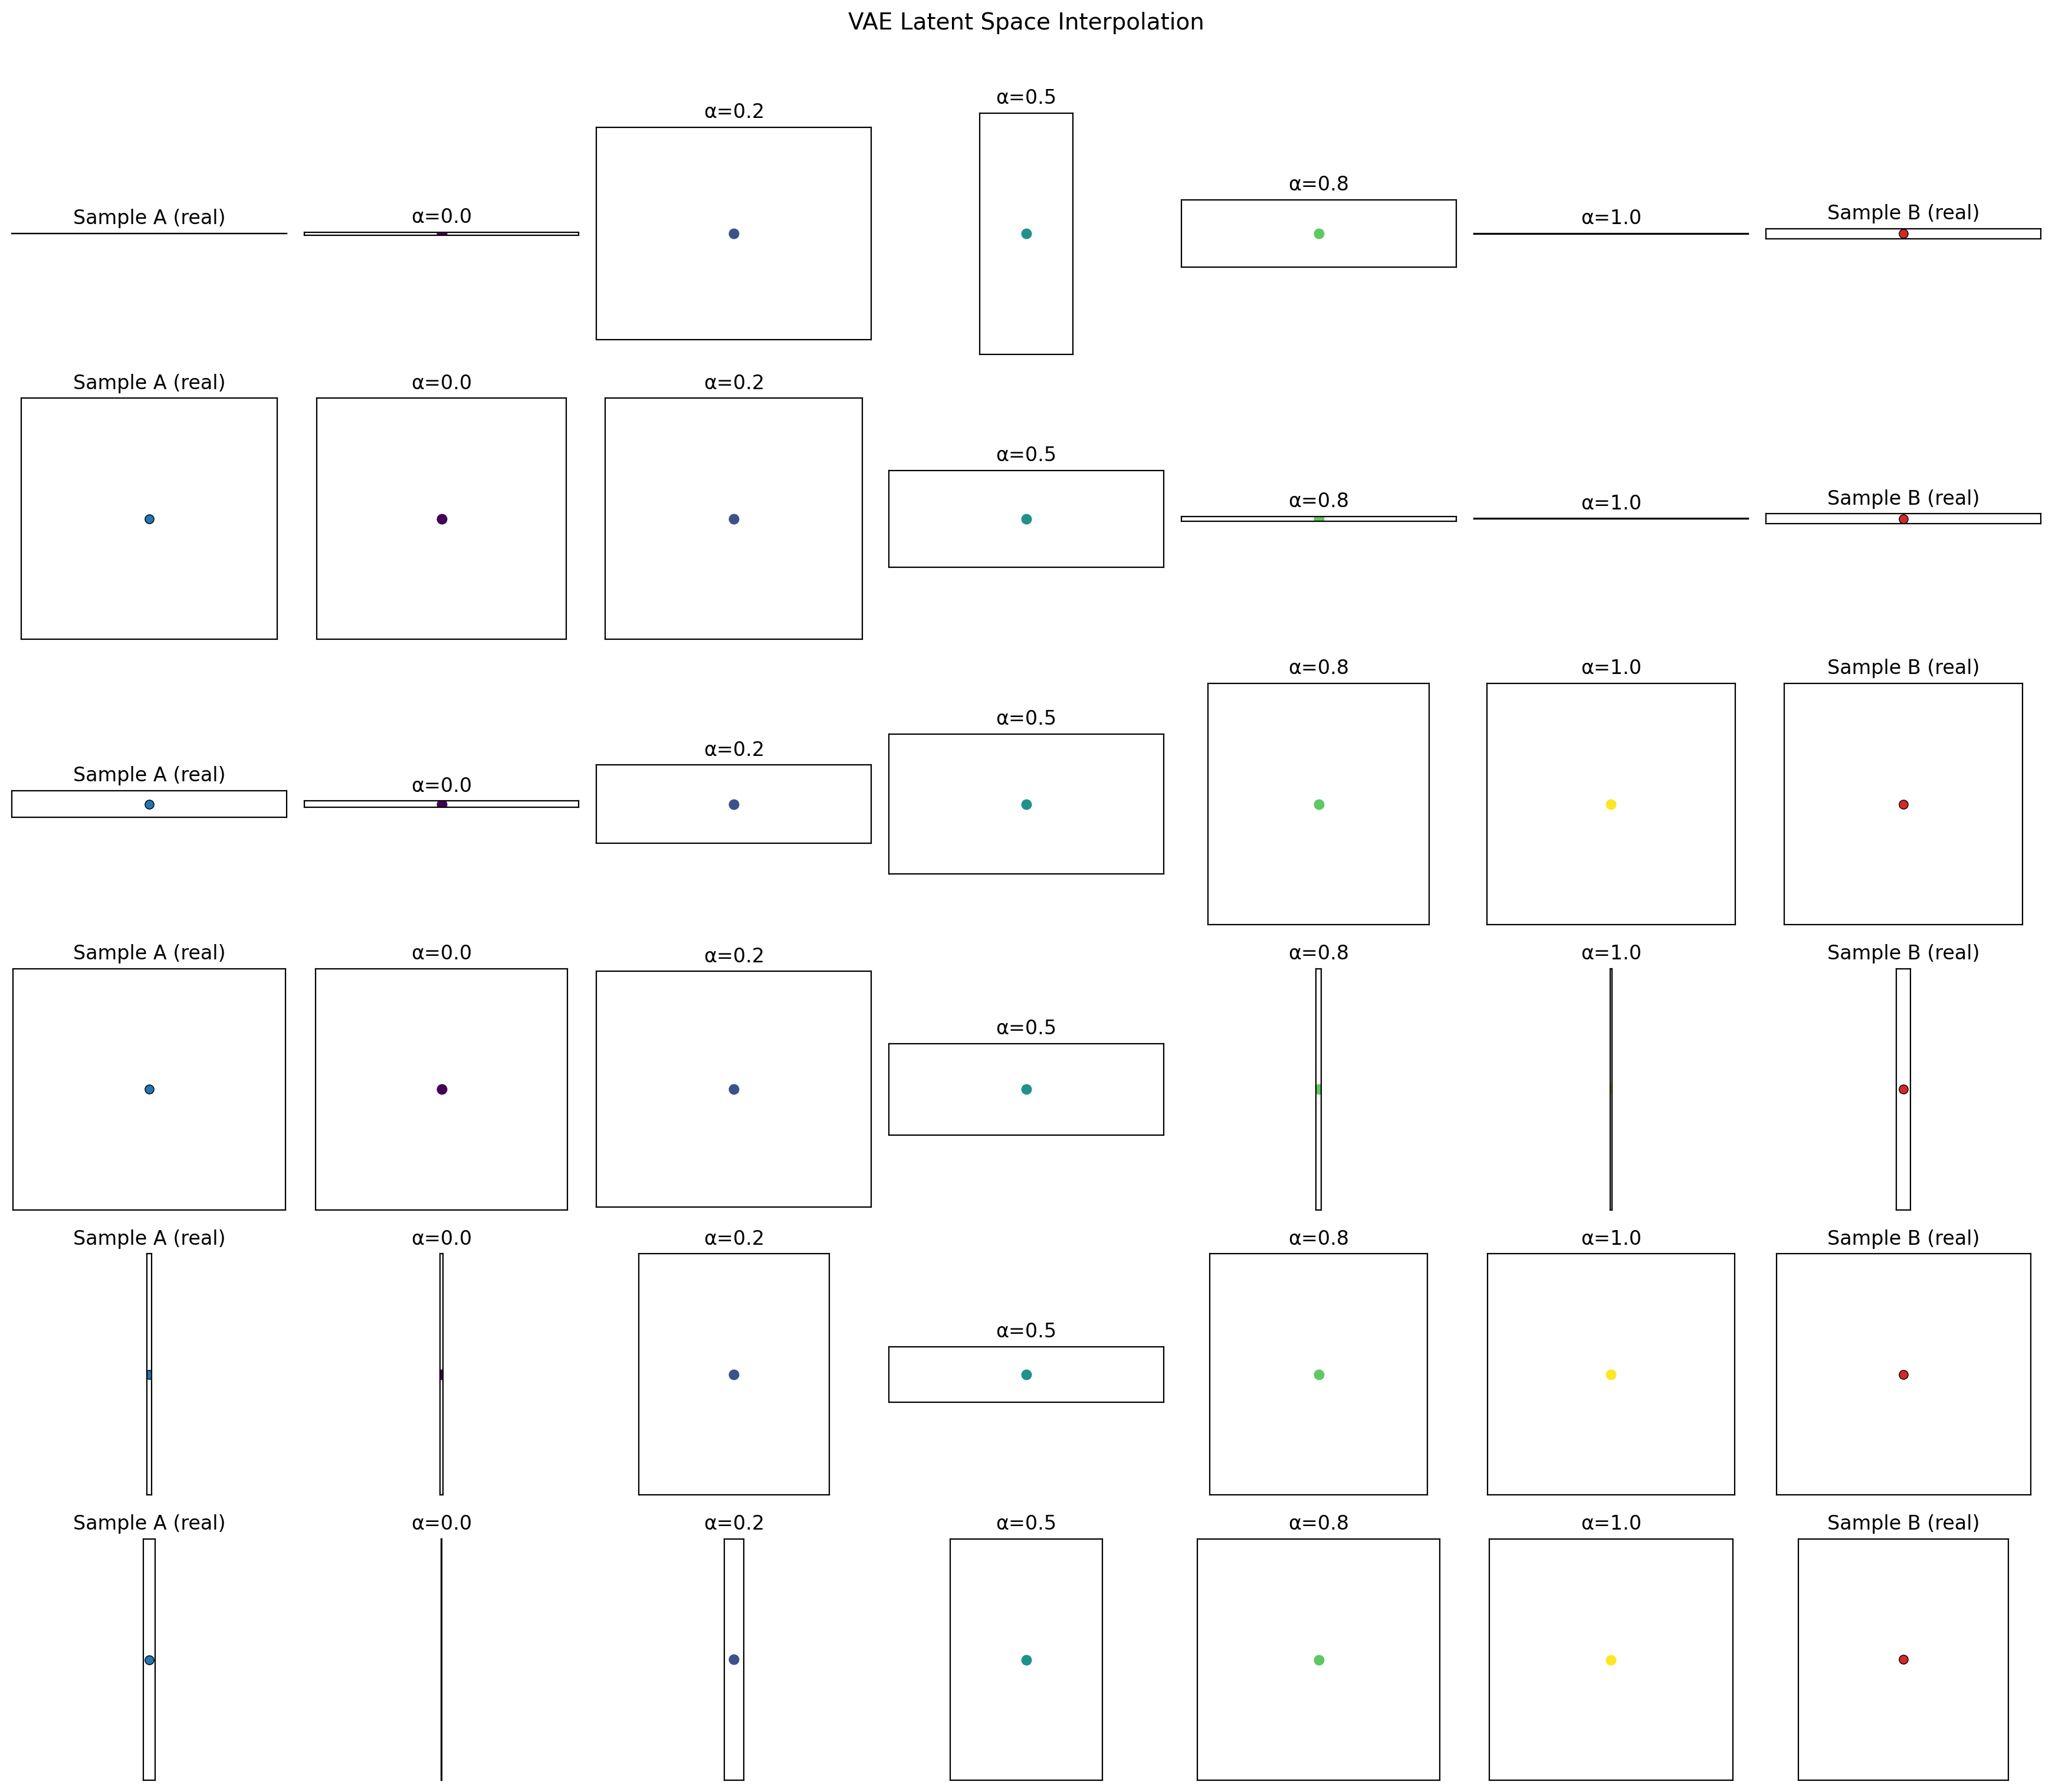
\includegraphics[width=\linewidth]{vae_gaussian_mixture_latent_interpolation.png}
    \caption{VAE on Gaussian Mixture: 潜空间插值}
\end{subfigure}
\caption{VAE 潜空间插值。每行展示了一对真实样本之间在潜空间中的线性插值轨迹。}
\end{figure}

\begin{figure}[H]
\centering
\begin{subfigure}[b]{0.48\textwidth}
    
\includegraphics[width=\linewidth]{diffusion_two_moons_enhanced_snapshots.png}
    \caption{DDPM on Two Moons: 十步去噪快照}
\end{subfigure}
\hfill
\begin{subfigure}[b]{0.48\textwidth}
    
\includegraphics[width=\linewidth]{diffusion_gaussian_mixture_enhanced_snapshots.png}
    \caption{DDPM on Gaussian Mixture: 十步去噪快照}
\end{subfigure}
\vspace{0.4em}
\begin{subfigure}[b]{0.48\textwidth}
    
\includegraphics[width=\linewidth]{diffusion_spiral_enhanced_snapshots.png}
    \caption{DDPM on Spiral: 十步去噪快照}
\end{subfigure}
\hfill
\begin{subfigure}[b]{0.48\textwidth}
    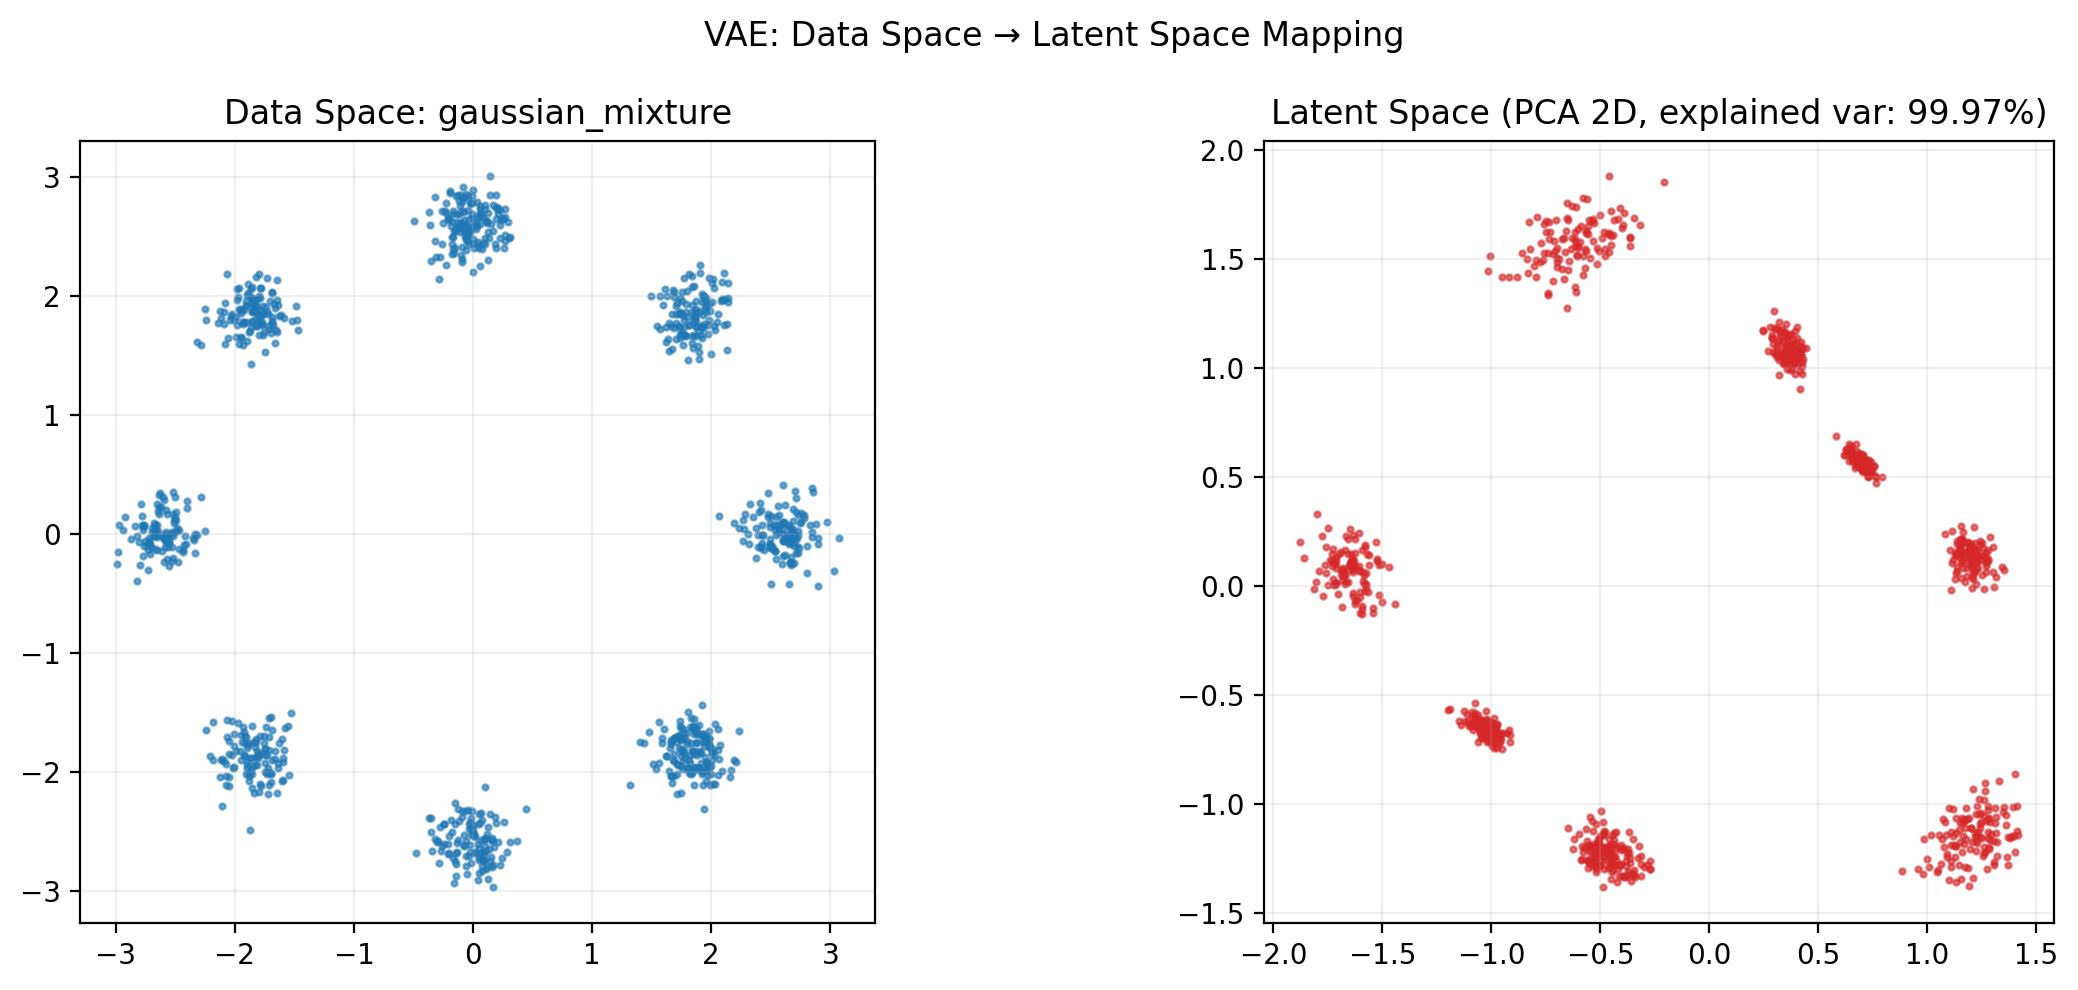
\includegraphics[width=\linewidth]{vae_gaussian_mixture_encoding_scatter.png}
    \caption{VAE on Gaussian Mixture: 编码散点}
\end{subfigure}
\caption{补充可视化：（a-c）各分布上的 DDPM 十步去噪快照；（d）VAE 编码器将数据空间映射到潜空间的可视化。}
\end{figure}

\begin{figure}[H]
\centering
\begin{subfigure}[b]{0.48\textwidth}
    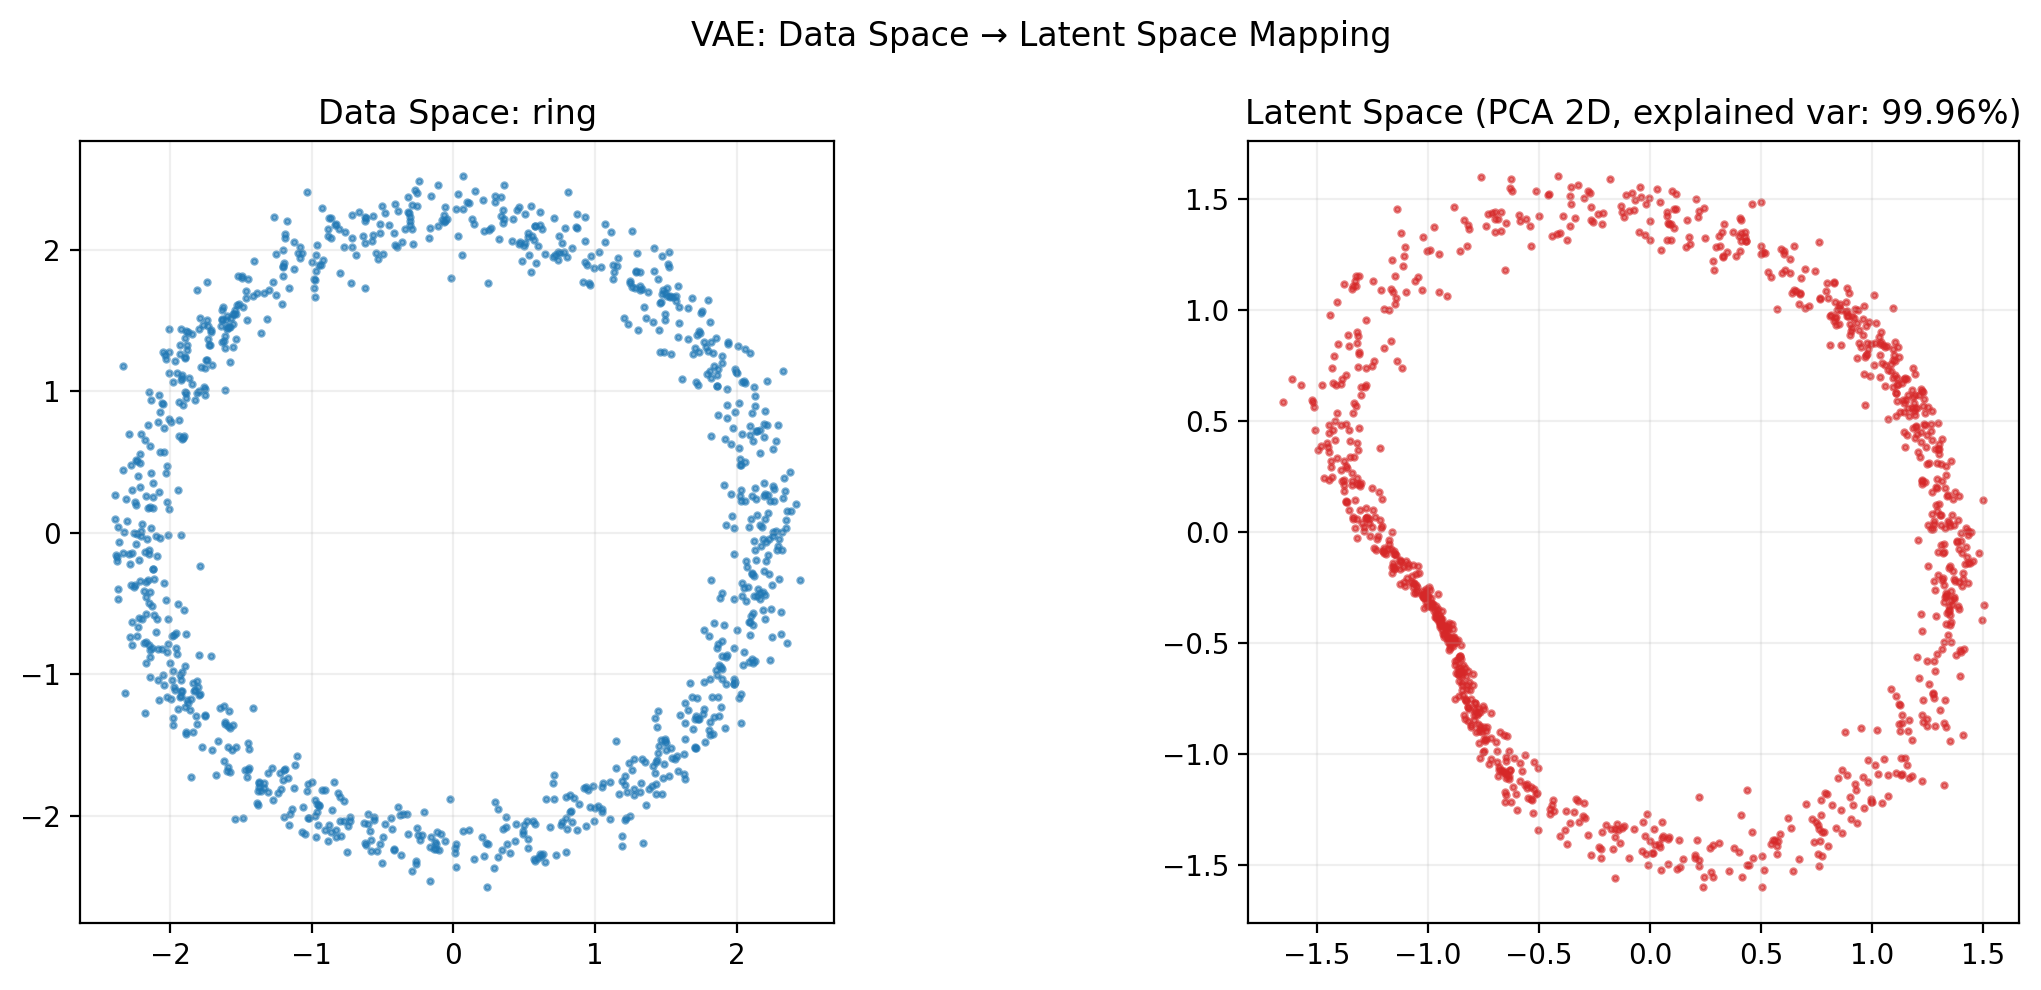
\includegraphics[width=\linewidth]{vae_ring_encoding_scatter.png}
    \caption{VAE on Ring: 编码散点}
\end{subfigure}
\hfill
\begin{subfigure}[b]{0.48\textwidth}
    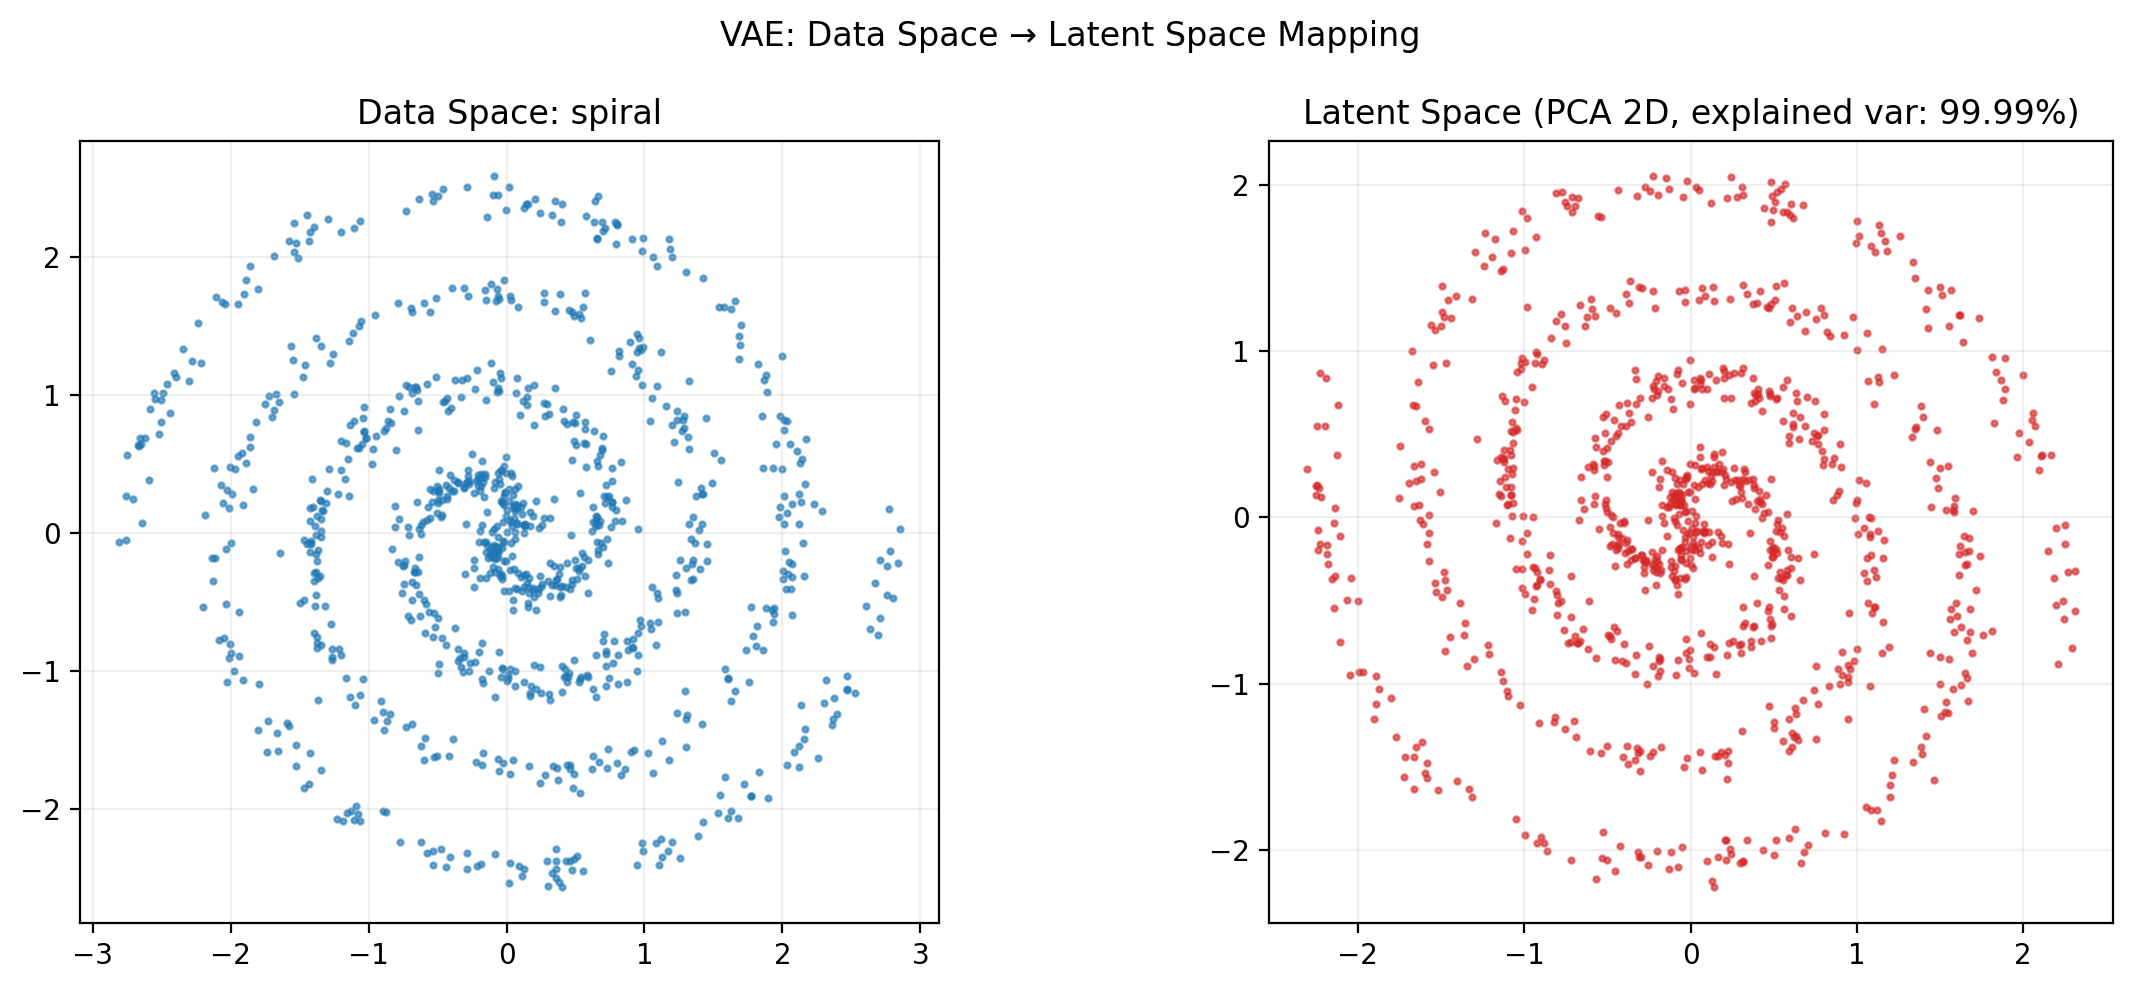
\includegraphics[width=\linewidth]{vae_spiral_encoding_scatter.png}
    \caption{VAE on Spiral: 编码散点}
\end{subfigure}
\vspace{0.4em}
\begin{subfigure}[b]{0.48\textwidth}
    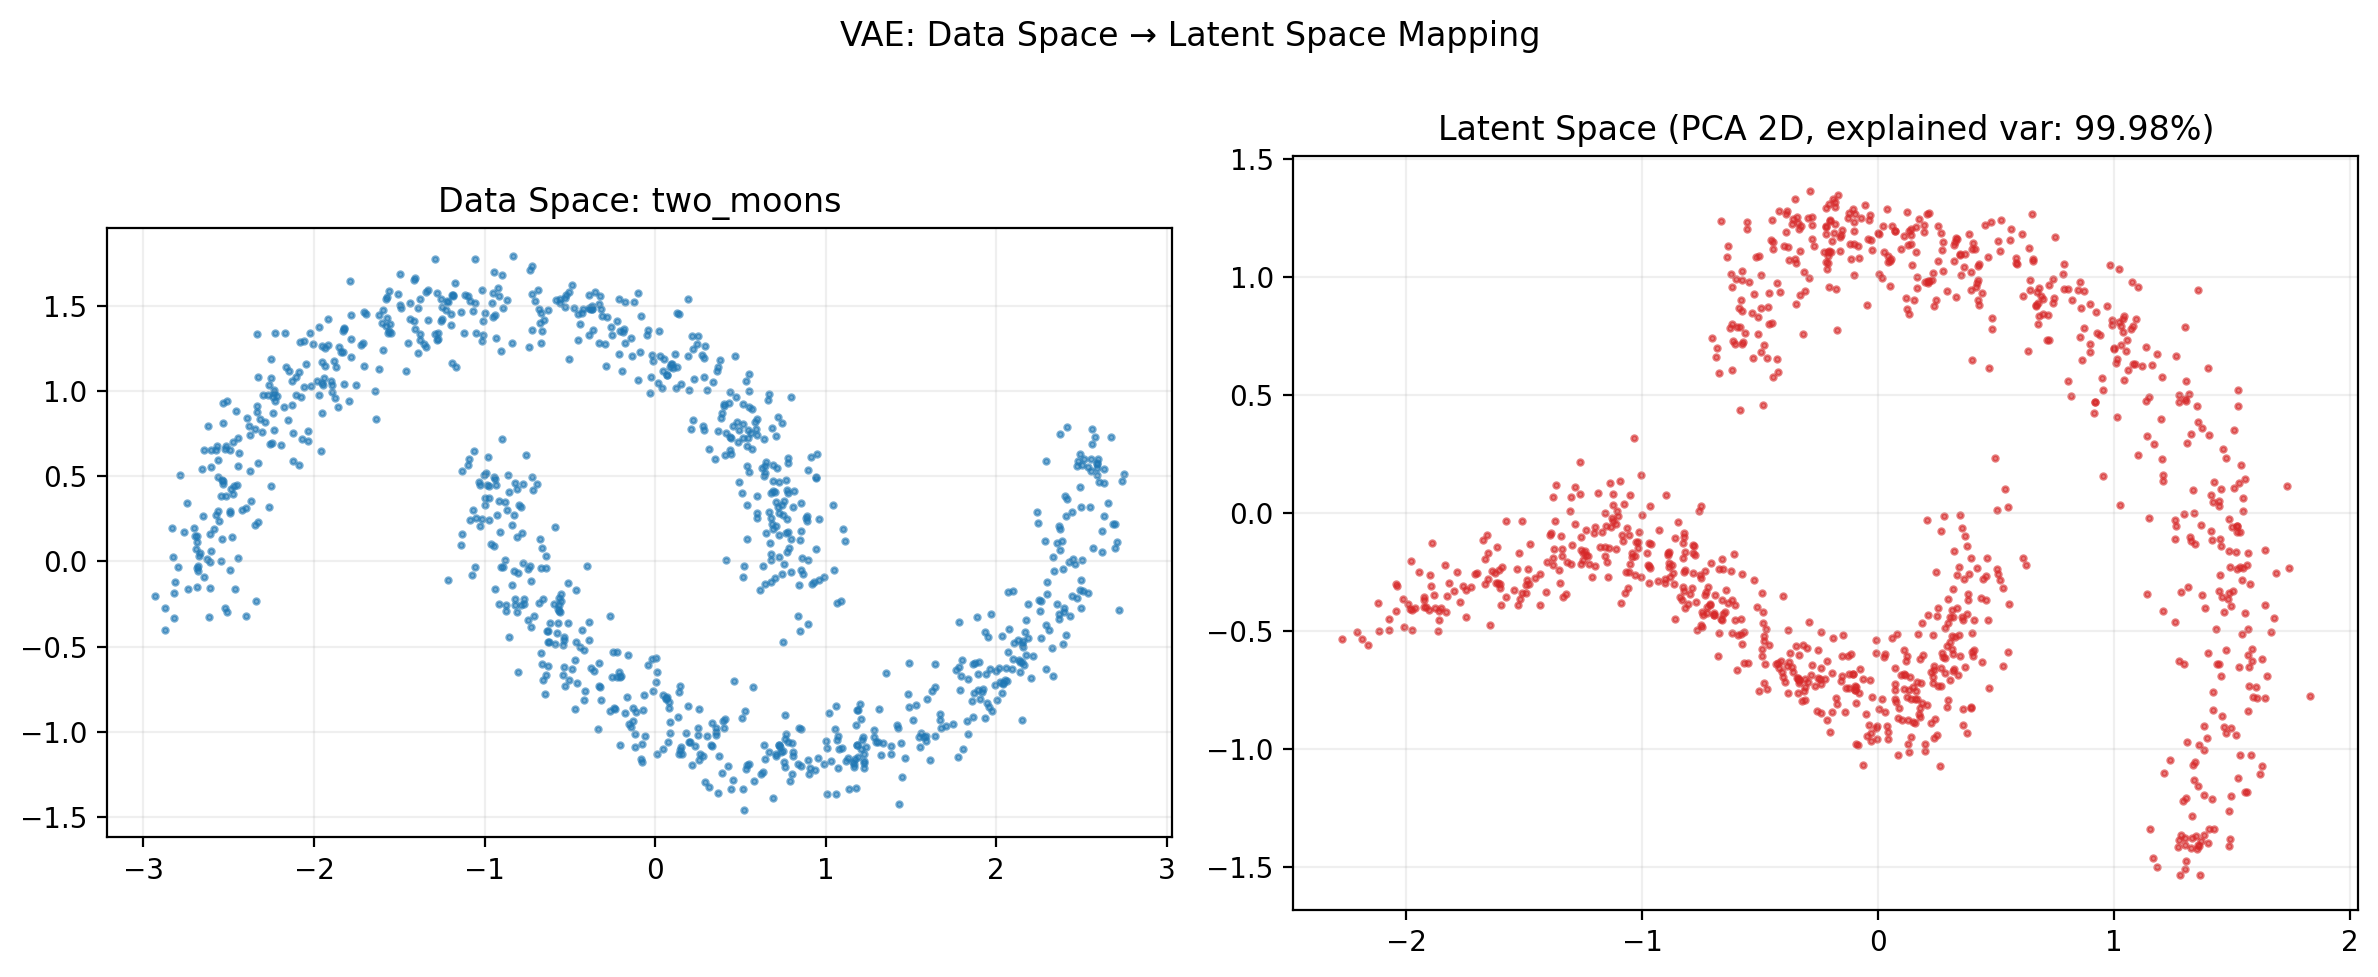
\includegraphics[width=\linewidth]{vae_two_moons_encoding_scatter.png}
    \caption{VAE on Two Moons: 编码散点}
\end{subfigure}
\hfill
\begin{subfigure}[b]{0.48\textwidth}
    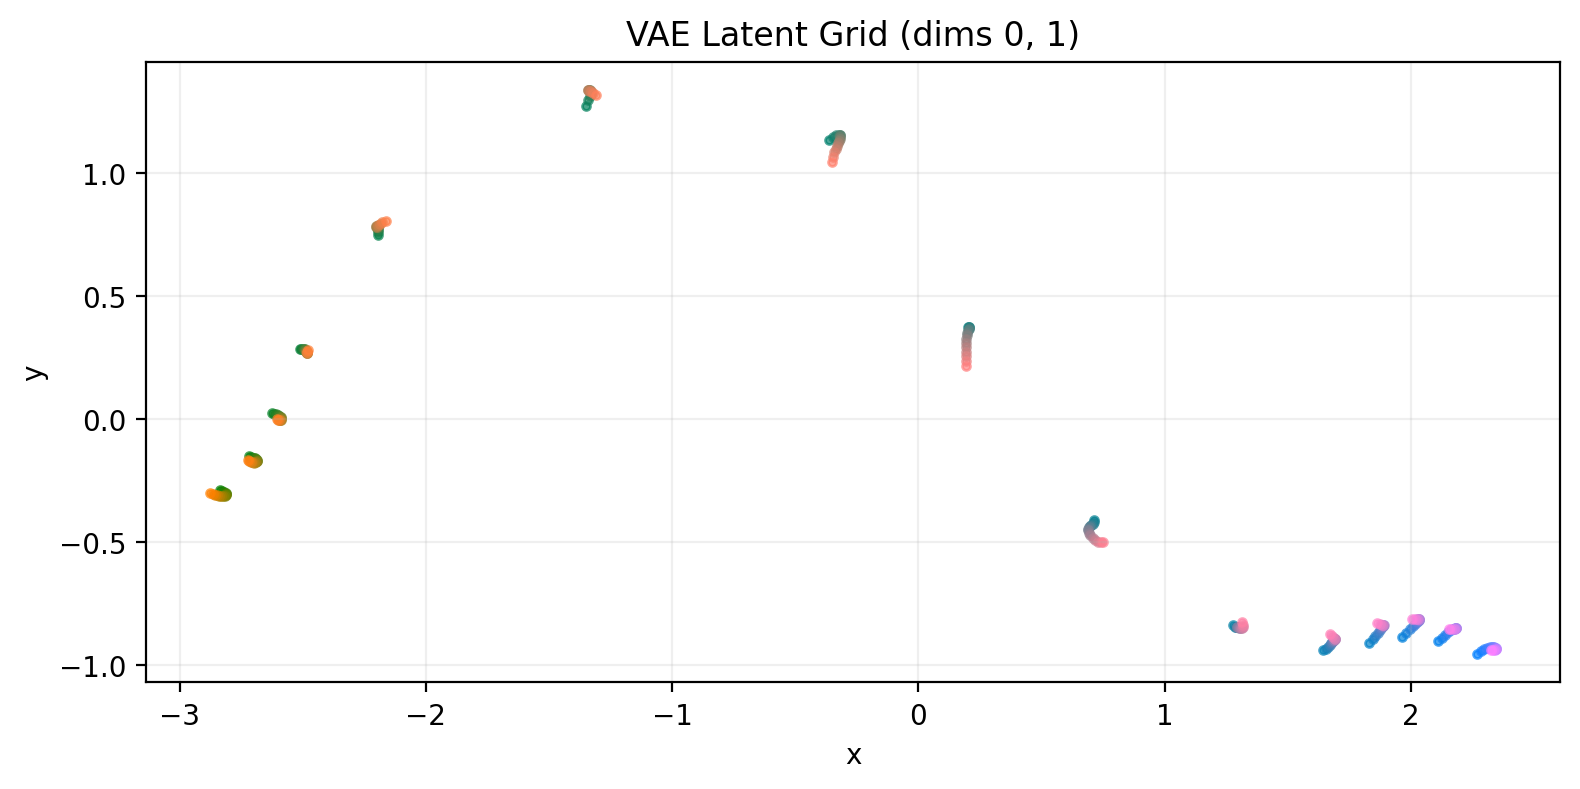
\includegraphics[width=\linewidth]{vae_two_moons_latent_grid.png}
    \caption{VAE on Two Moons: 潜空间网格}
\end{subfigure}
\caption{各分布上 VAE 的数据空间到潜空间的编码映射，以及 Two Moons 的潜空间网格遍历。}
\end{figure}

\section{完整实验数据}

\begin{table}[H]
\centering
\small
\caption{三类模型在四类分布上的完整评价指标（5 种子均值 $\pm$ 标准差）。KDE-NLL 和 GMM-NLL 为辅助似然代理指标。}
\label{tab:full-metrics}
\begin{tabular}{llccc}
\toprule
数据集 & 模型 & KDE-NLL $\downarrow$ & GMM-NLL $\downarrow$ & 训练时间/s \\
\midrule
\multirow{3}{*}{Gaussian Mixture}
    & VAE    & $4.849\pm0.005$ & $2.671\pm0.117$ & $2.40\pm0.20$ \\
    & DDPM   & $4.859\pm0.017$ & $\mathbf{2.258\pm0.100}$ & $\mathbf{2.92\pm0.08}$ \\
    & Flow   & $\mathbf{4.870\pm0.006}$ & $2.447\pm0.093$ & $18.51\pm0.37$ \\
\midrule
\multirow{3}{*}{Ring}
    & VAE    & $\mathbf{4.486\pm0.014}$ & $2.661\pm0.077$ & $\mathbf{2.16\pm0.21}$ \\
    & DDPM   & $4.535\pm0.008$ & $2.432\pm0.024$ & $2.42\pm0.09$ \\
    & Flow   & $4.546\pm0.001$ & $\mathbf{2.424\pm0.018}$ & $18.97\pm0.66$ \\
\midrule
\multirow{3}{*}{Two Moons}
    & VAE    & $\mathbf{3.736\pm0.010}$ & $3.106\pm0.255$ & $\mathbf{2.00\pm0.13}$ \\
    & DDPM   & $3.735\pm0.025$ & $\mathbf{2.296\pm0.036}$ & $2.42\pm0.20$ \\
    & Flow   & $3.794\pm0.011$ & $2.235\pm0.033$ & $18.76\pm0.32$ \\
\midrule
\multirow{3}{*}{Spiral}
    & VAE    & $\mathbf{3.674\pm0.020}$ & $3.081\pm0.015$ & $\mathbf{2.39\pm0.11}$ \\
    & DDPM   & $3.695\pm0.017$ & $3.108\pm0.011$ & $3.01\pm0.07$ \\
    & Flow   & $3.722\pm0.023$ & $\mathbf{3.053\pm0.010}$ & $18.90\pm0.26$ \\
\bottomrule
\end{tabular}
\end{table}

从补充指标来看，GMM-NLL 和 KDE-NLL 给出的排序与核心指标并不完全一致。例如，DDPM 在 Gaussian Mixture 和 Ring 上的 GMM-NLL 均为最优，但在核心 MMD 指标上却不及 Flow。这正说明了多个互补指标联合使用的必要性：概率密度代理和几何分布一致性捕捉的是生成质量的不同侧面，不存在某个单一的"万能指标"。

\clearpage
% ===================== 参考文献 =====================
\begin{thebibliography}{99}

\bibitem{lai2025principles}
Lai, Chieh-Hsin and Song, Yang and Kim, Dongjun and Mitsufuji, Yuki and Ermon, Stefano.
\newblock The principles of diffusion models.
\newblock \emph{arXiv preprint arXiv:2510.21890LR)}, 2025.


\end{thebibliography}

\end{document}
